% Options for packages loaded elsewhere
\PassOptionsToPackage{unicode}{hyperref}
\PassOptionsToPackage{hyphens}{url}
%
\documentclass[
]{article}
\usepackage{lmodern}
\usepackage{amssymb,amsmath}
\usepackage{ifxetex,ifluatex}
\ifnum 0\ifxetex 1\fi\ifluatex 1\fi=0 % if pdftex
  \usepackage[T1]{fontenc}
  \usepackage[utf8]{inputenc}
  \usepackage{textcomp} % provide euro and other symbols
\else % if luatex or xetex
  \usepackage{unicode-math}
  \defaultfontfeatures{Scale=MatchLowercase}
  \defaultfontfeatures[\rmfamily]{Ligatures=TeX,Scale=1}
\fi
% Use upquote if available, for straight quotes in verbatim environments
\IfFileExists{upquote.sty}{\usepackage{upquote}}{}
\IfFileExists{microtype.sty}{% use microtype if available
  \usepackage[]{microtype}
  \UseMicrotypeSet[protrusion]{basicmath} % disable protrusion for tt fonts
}{}
\makeatletter
\@ifundefined{KOMAClassName}{% if non-KOMA class
  \IfFileExists{parskip.sty}{%
    \usepackage{parskip}
  }{% else
    \setlength{\parindent}{0pt}
    \setlength{\parskip}{6pt plus 2pt minus 1pt}}
}{% if KOMA class
  \KOMAoptions{parskip=half}}
\makeatother
\usepackage{xcolor}
\IfFileExists{xurl.sty}{\usepackage{xurl}}{} % add URL line breaks if available
\IfFileExists{bookmark.sty}{\usepackage{bookmark}}{\usepackage{hyperref}}
\hypersetup{
  pdftitle={A Bioconductor workflow for the Bayesian analysis of spatial proteomics},
  hidelinks,
  pdfcreator={LaTeX via pandoc}}
\urlstyle{same} % disable monospaced font for URLs
\usepackage[margin=1in]{geometry}
\usepackage{color}
\usepackage{fancyvrb}
\newcommand{\VerbBar}{|}
\newcommand{\VERB}{\Verb[commandchars=\\\{\}]}
\DefineVerbatimEnvironment{Highlighting}{Verbatim}{commandchars=\\\{\}}
% Add ',fontsize=\small' for more characters per line
\usepackage{framed}
\definecolor{shadecolor}{RGB}{248,248,248}
\newenvironment{Shaded}{\begin{snugshade}}{\end{snugshade}}
\newcommand{\AlertTok}[1]{\textcolor[rgb]{0.94,0.16,0.16}{#1}}
\newcommand{\AnnotationTok}[1]{\textcolor[rgb]{0.56,0.35,0.01}{\textbf{\textit{#1}}}}
\newcommand{\AttributeTok}[1]{\textcolor[rgb]{0.77,0.63,0.00}{#1}}
\newcommand{\BaseNTok}[1]{\textcolor[rgb]{0.00,0.00,0.81}{#1}}
\newcommand{\BuiltInTok}[1]{#1}
\newcommand{\CharTok}[1]{\textcolor[rgb]{0.31,0.60,0.02}{#1}}
\newcommand{\CommentTok}[1]{\textcolor[rgb]{0.56,0.35,0.01}{\textit{#1}}}
\newcommand{\CommentVarTok}[1]{\textcolor[rgb]{0.56,0.35,0.01}{\textbf{\textit{#1}}}}
\newcommand{\ConstantTok}[1]{\textcolor[rgb]{0.00,0.00,0.00}{#1}}
\newcommand{\ControlFlowTok}[1]{\textcolor[rgb]{0.13,0.29,0.53}{\textbf{#1}}}
\newcommand{\DataTypeTok}[1]{\textcolor[rgb]{0.13,0.29,0.53}{#1}}
\newcommand{\DecValTok}[1]{\textcolor[rgb]{0.00,0.00,0.81}{#1}}
\newcommand{\DocumentationTok}[1]{\textcolor[rgb]{0.56,0.35,0.01}{\textbf{\textit{#1}}}}
\newcommand{\ErrorTok}[1]{\textcolor[rgb]{0.64,0.00,0.00}{\textbf{#1}}}
\newcommand{\ExtensionTok}[1]{#1}
\newcommand{\FloatTok}[1]{\textcolor[rgb]{0.00,0.00,0.81}{#1}}
\newcommand{\FunctionTok}[1]{\textcolor[rgb]{0.00,0.00,0.00}{#1}}
\newcommand{\ImportTok}[1]{#1}
\newcommand{\InformationTok}[1]{\textcolor[rgb]{0.56,0.35,0.01}{\textbf{\textit{#1}}}}
\newcommand{\KeywordTok}[1]{\textcolor[rgb]{0.13,0.29,0.53}{\textbf{#1}}}
\newcommand{\NormalTok}[1]{#1}
\newcommand{\OperatorTok}[1]{\textcolor[rgb]{0.81,0.36,0.00}{\textbf{#1}}}
\newcommand{\OtherTok}[1]{\textcolor[rgb]{0.56,0.35,0.01}{#1}}
\newcommand{\PreprocessorTok}[1]{\textcolor[rgb]{0.56,0.35,0.01}{\textit{#1}}}
\newcommand{\RegionMarkerTok}[1]{#1}
\newcommand{\SpecialCharTok}[1]{\textcolor[rgb]{0.00,0.00,0.00}{#1}}
\newcommand{\SpecialStringTok}[1]{\textcolor[rgb]{0.31,0.60,0.02}{#1}}
\newcommand{\StringTok}[1]{\textcolor[rgb]{0.31,0.60,0.02}{#1}}
\newcommand{\VariableTok}[1]{\textcolor[rgb]{0.00,0.00,0.00}{#1}}
\newcommand{\VerbatimStringTok}[1]{\textcolor[rgb]{0.31,0.60,0.02}{#1}}
\newcommand{\WarningTok}[1]{\textcolor[rgb]{0.56,0.35,0.01}{\textbf{\textit{#1}}}}
\usepackage{graphicx,grffile}
\makeatletter
\def\maxwidth{\ifdim\Gin@nat@width>\linewidth\linewidth\else\Gin@nat@width\fi}
\def\maxheight{\ifdim\Gin@nat@height>\textheight\textheight\else\Gin@nat@height\fi}
\makeatother
% Scale images if necessary, so that they will not overflow the page
% margins by default, and it is still possible to overwrite the defaults
% using explicit options in \includegraphics[width, height, ...]{}
\setkeys{Gin}{width=\maxwidth,height=\maxheight,keepaspectratio}
% Set default figure placement to htbp
\makeatletter
\def\fps@figure{htbp}
\makeatother
\setlength{\emergencystretch}{3em} % prevent overfull lines
\providecommand{\tightlist}{%
  \setlength{\itemsep}{0pt}\setlength{\parskip}{0pt}}
\setcounter{secnumdepth}{-\maxdimen} % remove section numbering

\title{A Bioconductor workflow for the Bayesian analysis of spatial proteomics}
\author{true \and true \and true \and true \and true}
\date{}

\begin{document}
\maketitle
\begin{abstract}
Knowledge of the subcellular location of a protein gives valuable
insight into its function. The field of spatial proteomics has become
increasingly popular due to improved multiplexing capabilities in
high-throughput mass spectrometry, which have made it possible to
systematically localise thousands of proteins per experiment. In
parallel with these experimental advances, improved methods for
analysing spatial proteomics data have also been developed. In this
workflow, we demonstrate using \texttt{pRoloc} to perform Bayesian
analysis of spatial proteomics data. We detail the software
infrastructure and then provide step-by-step guidance of the analysis,
including setting up a pipeline, assessing convergence, and interpreting
downstream results. In several places we provide additional details on
Bayesian analysis to provide users with a holistic view of Bayesian
analysis for spatial proteomics data.
\end{abstract}

\newcommand{\diag}{\mathop{\mathrm{diag}}}

\textbf{R version}: R version 4.0.0 (2020-04-24)

\textbf{Bioconductor version}: 3.11

\hypertarget{introduction}{%
\section{Introduction}\label{introduction}}

Determining the spatial subcellular distribution of proteins enables
novel insight into protein function (Crook et al. 2018). Many proteins
function within a single location within the cell; however, it is
estimated that up to half of the proteome is thought to reside in
multiple locations, with some of these undergoing dynamic relocalisation
(Thul et al. 2017). These phenomena lead to variability and uncertainty
in robustly assigning proteins to a unique localisation. Functional
compartmentalisation of proteins allows the cell to control biomolecular
pathways and biochemical processes within the cell. Therefore, proteins
with multiple localisations may have multiple functional roles (Jeffery
2009). Machine learning algorithms that fail to quantify uncertainty are
unable to draw deeper insight into understanding cell biology from mass
spectrometry (MS)-based spatial proteomics experiments. Hence,
quantifying uncertainty allows us to make rigorous assessments of
protein subcellular localisation and multi-localisation.

For proteins to carry out their functional role they must be localised
to the correct subcellular compartment, ensuring the biochemical
conditions for desired molecular interactions are met (Gibson 2009).
Many pathologies, including cancer and obesity are characterised by
protein mis-localisations (Olkkonen and Ikonen 2006; Laurila and Vihinen
2009; Luheshi, Crowther, and Dobson 2008; De Matteis and Luini 2011;
Cody, Iampietro, and Lécuyer 2013; Kau, Way, and Silver 2004; Rodriguez,
Au, and Henderson 2004; Latorre et al. 2005; Shin et al. 2013; Siljee et
al. 2018). High-throughput spatial proteomics technologies have seen
rapid improvement over the last decade and now a single experiment can
provide spatial information on thousands of proteins at once (Dunkley et
al. 2006; Foster et al. 2006; Christoforou et al. 2016; Geladaki et al.
2019). As a result of these spatial proteomics technologies many
biological systems have been characterised (Dunkley et al. 2006; Tan et
al. 2009; Hall et al. 2009; Breckels et al. 2013; Christoforou et al.
2016; Thul et al. 2017). The popularity of such methods is now evident
with many new studies in recent years (Christoforou et al. 2016;
Beltran, Mathias, and Cristea 2016; Jadot et al. 2017; Itzhak et al.
2017; Mendes et al. 2017; Hirst et al. 2018; Davies et al. 2018; Orre et
al. 2019; Nightingale et al. 2019).

Mass spectrometry-based spatial proteomic experiments begin with the
gentle lysis of a population of cells in a fashion that maintains the
integrity of the organelles. To separate cellular content a variety of
methods are available, including equilibrium gradient-density separation
(Christoforou et al. 2016; Mulvey et al. 2017) or differential
centrifugation (Geladaki et al. 2019). For example, in hyperLOPIT
(Mulvey et al. 2017) cell lysis is followed by the separation of
subcellular components along a continuous density gradient based on
their buoyant density. Discrete fractions along this gradient are then
collected, and protein distributions revealing organelle specific
correlation profiles within the fractions are achieved using high
accuracy MS. Proteins from the dataset are then manually annotated with
well-documented single localisations curated from the literature,
referred to as organelle markers (see Gatto et al.~(Gatto, Breckels, et
al. 2014a)). A prediction model is then trained from these markers to
create a classifier, which assigns proteins with unknown localisation to
a sub-cellular niche (Gatto, Breckels, et al. 2014a).

Bayesian approaches to machine learning and statistics can provide more
insight, by providing uncertainty quantification (Gelman et al. 1995).
In a parametric Bayesian setting, a parametric model is proposed, along
with a statement about our prior beliefs of the model parameters. Bayes'
theorem tells us how to update the prior distribution of the parameters
to obtain the posterior distribution of the parameters after observing
the data. It is the posterior distribution which quantifies the
uncertainty in the parameters. This contrasts from a maximum-likelihood
approach where we obtain only a point estimate of the parameters.

Adopting a Bayesian framework for data analysis, though of much interest
to experimentalists, can be challenging. Once we have specified a
probabilistic model, computational approaches are typically used to
obtain the posterior distribution upon observation of the data. These
algorithms can have parameters that require tuning and a variety of
settings, hindering their practical use by those not familiar with
Bayesian methodology. Even once the algorithms have been correctly
set-up, assessments of convergence and guidance on how to interpret the
results are often sparse. This workflow presents a Bayesian analysis of
spatial proteomics to elucidate the process for practitioners. Our
workflow also provides a template for others interested in designing
tools for the biological community which rely on Bayesian inference.

Our model for the data is the t-augmented Gaussian mixture (TAGM) model
proposed in (Crook et al. 2018). Crook et al. (2018) provide a detailed
description of the model, rigorous comparisons and testing on many
spatial proteomics datasets. In addition, they include a case study of a
hyperLOPIT experiment performed on mouse pluripotent stem cells
(Christoforou et al. 2016; Mulvey et al. 2017). Revisiting these details
is not the purpose of this computational protocol; rather we present how
to correctly use the software and provide step-by-step guidance for
interpreting the results.

In brief, the TAGM model posits that each annotated sub-cellular niche
can be modelled using a Gaussian distribution. Thus the full complement
of proteins within the cell is captured as a mixture of Gaussians. The
highly dynamic nature of the cell means that many proteins are not well
captured by any of these multivariate Gaussian distributions, and thus
the model also includes an outlier component, which is mathematically
described as a multivariate student's t distribution. The heavy tails of
the t distribution allow it to better capture dispersed proteins. The
outlier component is included to avoid allocating proteins which are far
from any annotated subcellular niche. These proteins can be interpreted
in multiple ways: they could be part of an unannotated subcellular
niche, they could reside in multiple locations, they could have highly
variable sub-cellular niches or they could have been poorly quantified.

There are two approaches to perform inference in the TAGM model. The
first, which we refer to as TAGM MAP, allows us to obtain \emph{maximum
a posteriori} estimates of posterior localisation probabilities; that
is, the modal posterior probability that a protein localises to that
class. This approach uses the expectation-maximisation (EM) algorithm to
perform inference (Dempster, Laird, and Rubin 1977). Whilst this is an
interpretable summary of the TAGM model, it only provides point
estimates. For a richer analysis, we also present a Markov-chain
Monte-Carlo (MCMC) method to perform fully Bayesian inference in our
model, allowing us to obtain full posterior localisation distributions.
This method is referred to as TAGM MCMC throughout the text.

This workflow begins with a brief review of some of the basic features
of mass spectrometry-based spatial proteomics data, including our
state-of-the-art computational infrastructure and bespoke software
suite. We then present each method in turn, detailing how to obtain high
quality results. We provide an extended discussion of the TAGM MCMC
method to highlight some of the challenges that may arise when applying
this method. This includes how to assess convergence of MCMC methods, as
well as methods for manipulating the output. We then take the processed
output and explain how to interpret the results, as well as providing
some tools for visualisation. We conclude with some remarks and
directions for the future. Source code for this workflow, including code
used to generate tables and figures, is available on
\href{https://github.com/ococrook/TAGMworkflow}{GitHub} (Oliver M. Crook
et al. 2019)

\hypertarget{getting-started-and-infrastructure}{%
\section{Getting started and
infrastructure}\label{getting-started-and-infrastructure}}

In this workflow, we are using version 1.23.2 of \texttt{pRoloc} (Gatto,
Breckels, et al. 2014b). The package \texttt{pRoloc} contains algorithms
and methods for analysing spatial proteomics data, building on the
\texttt{MSnSet} structure provided in \texttt{MSnbase}. The
\texttt{pRolocdata} package provides many annotated datasets from a
variety of species and experimental procedures. The following code
chunks install and load the suite of packages require for the analysis.

\begin{Shaded}
\begin{Highlighting}[]
\ControlFlowTok{if}\NormalTok{ (}\OperatorTok{!}\KeywordTok{require}\NormalTok{(}\StringTok{"BiocManager"}\NormalTok{))}
    \KeywordTok{install.package}\NormalTok{(}\StringTok{"BiocManager"}\NormalTok{)}
\NormalTok{BiocManager}\OperatorTok{::}\KeywordTok{install}\NormalTok{(}\KeywordTok{c}\NormalTok{(}\StringTok{"pRoloc"}\NormalTok{, }\StringTok{"pRolocdata"}\NormalTok{))}
\end{Highlighting}
\end{Shaded}

\begin{Shaded}
\begin{Highlighting}[]
\KeywordTok{library}\NormalTok{(}\StringTok{"pRoloc"}\NormalTok{)}
\end{Highlighting}
\end{Shaded}

\begin{verbatim}
## 
## This is pRoloc version 1.28.0 
##   Visit https://lgatto.github.io/pRoloc/ to get started.
\end{verbatim}

\begin{verbatim}
## 
## Attaching package: 'pRoloc'
\end{verbatim}

\begin{verbatim}
## The following object is masked _by_ '.GlobalEnv':
## 
##     spatial2D
\end{verbatim}

\begin{Shaded}
\begin{Highlighting}[]
\KeywordTok{library}\NormalTok{(}\StringTok{"pRolocdata"}\NormalTok{)}
\end{Highlighting}
\end{Shaded}

\begin{verbatim}
## 
## This is pRolocdata version 1.26.0.
## Use 'pRolocdata()' to list available data sets.
\end{verbatim}

We assume that we have an MS-based spatial proteomics dataset contained
in a \texttt{MSnSet} structure. For information on how to import data,
perform basic data processing, quality control, supervised machine
learning and transfer learning we refer the reader to (Breckels, Mulvey,
et al. 2016). Here, we start by loading a spatial proteomics dataset on
mouse E14TG2a embryonic stem cells (Breckels, Holden, et al. 2016). The
LOPIT protocol (Dunkley et al. 2004, 2006) was used and the normalised
intensity of proteins from eight iTRAQ 8-plex labelled fraction are
provided. The methods provided here are independent of labelling
procedure, fractionation process or workflow. Examples of valid
experimental protocols are LOPIT (Dunkley et al. 2004), hyperLOPIT
(Christoforou et al. 2016; Mulvey et al. 2017), label-free methods such
as PCP (Foster et al. 2006), and when fractionation is performed by
differential centrifugation (Itzhak et al. 2016; Geladaki et al. 2019).

In the code chunk below, we load the aforementioned dataset. The
printout demonstrates that this experiment quantified 2031 proteins over
8 fractions.

\begin{Shaded}
\begin{Highlighting}[]
\KeywordTok{data}\NormalTok{(}\StringTok{"E14TG2aR"}\NormalTok{) }\CommentTok{# load experimental data}
\NormalTok{E14TG2aR}
\end{Highlighting}
\end{Shaded}

\begin{verbatim}
## MSnSet (storageMode: lockedEnvironment)
## assayData: 2031 features, 8 samples 
##   element names: exprs 
## protocolData: none
## phenoData
##   sampleNames: n113 n114 ... n121 (8 total)
##   varLabels: Fraction.information
##   varMetadata: labelDescription
## featureData
##   featureNames: Q62261 Q9JHU4 ... Q9EQ93 (2031 total)
##   fvarLabels: Uniprot.ID UniprotName ... markers (8 total)
##   fvarMetadata: labelDescription
## experimentData: use 'experimentData(object)'
## Annotation:  
## - - - Processing information - - -
## Loaded on Thu Jul 16 15:02:29 2015. 
## Normalised to sum of intensities. 
## Added markers from  'mrk' marker vector. Thu Jul 16 15:02:29 2015 
##  MSnbase version: 1.17.12
\end{verbatim}

In figure @ref(fig:e14pca1), we can visualise the mouse stem cell
dataset using the \texttt{plot2D} function. We observe that some of the
organelle classes overlap and this is a typical feature of biological
datasets. Thus, it is vital to perform uncertainty quantification when
analysing biological data.

\begin{Shaded}
\begin{Highlighting}[]
\KeywordTok{plot2D}\NormalTok{(E14TG2aR)}
\KeywordTok{addLegend}\NormalTok{(E14TG2aR, }\DataTypeTok{where =} \StringTok{"topleft"}\NormalTok{, }\DataTypeTok{cex =} \FloatTok{0.6}\NormalTok{)}
\end{Highlighting}
\end{Shaded}

\begin{figure}
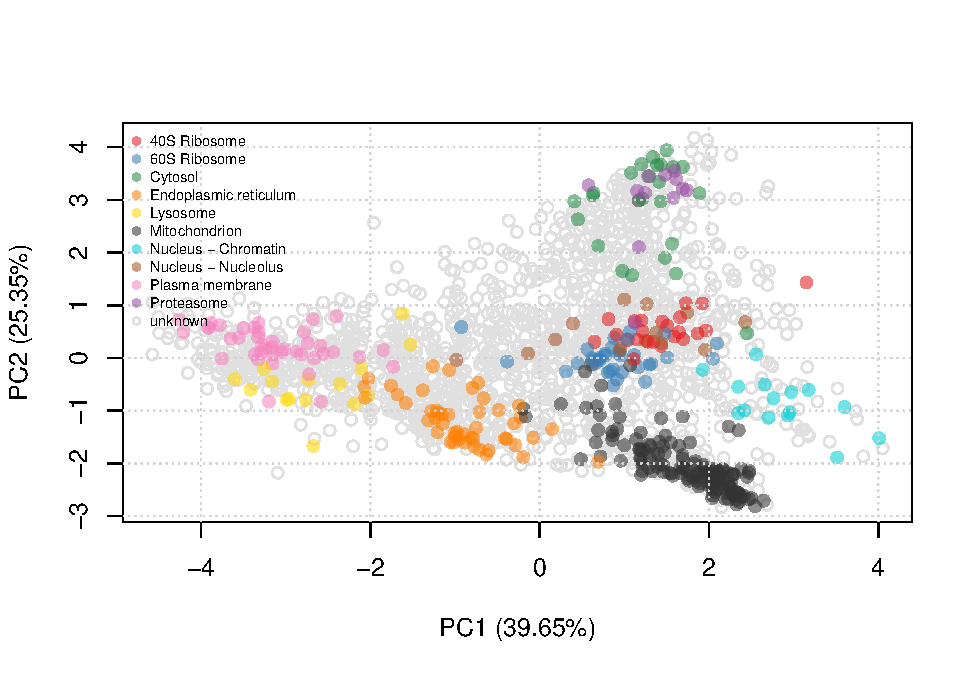
\includegraphics[width=0.8\linewidth]{F1000TAGMworkflow_rev1_files/figure-latex/e14pca1-1} \caption{The first two principal component of a mouse embryonic stem cell dataset [@Breckels:2016]. Each pointer represents a protein and marker proteins are coloured according to their localisation. Proteins with unknown localisation are coloured grey.}\label{fig:e14pca1}
\end{figure}

\hypertarget{methods-tagm-map}{%
\section{\texorpdfstring{Methods: \emph{TAGM
MAP}}{Methods: TAGM MAP}}\label{methods-tagm-map}}

\hypertarget{introduction-to-tagm-map}{%
\subsection{Introduction to TAGM MAP}\label{introduction-to-tagm-map}}

We can use \emph{maximum a posteriori} (MAP) estimation to perform
Bayesian parameter estimation for our model. The \emph{maximum a
posteriori} estimate is the mode of the posterior distribution and can
be used to provide a point estimate summary of the posterior
localisation probabilities. In contrast to TAGM MCMC (see later), it
does not provide samples from the posterior distribution, however it
allows faster inference by using an extended version of the
expectation-maximisation (EM) algorithm. The EM algorithm iterates
between an expectation step and a maximisation step. This allows us to
find parameters which maximise the logarithm of the posterior density,
in the presence of latent (unobserved) variables. The EM algorithm is
guaranteed to converge to a local mode. The code chunk below executes
the \texttt{tagmMapTrain} function for a default of 100 iterations. We
use the default priors for simplicity and convenience, however they can
be changed, which we explain in a later section. The output is an object
of class \texttt{MAPParams}, that captures the details of the TAGM MAP
model.

\begin{Shaded}
\begin{Highlighting}[]
\KeywordTok{set.seed}\NormalTok{(}\DecValTok{2}\NormalTok{)}
\NormalTok{mappars <-}\StringTok{ }\KeywordTok{tagmMapTrain}\NormalTok{(E14TG2aR)}
\end{Highlighting}
\end{Shaded}

\begin{verbatim}
## co-linearity detected; a small multiple of
##               the identity was added to the covariance
\end{verbatim}

\begin{Shaded}
\begin{Highlighting}[]
\NormalTok{mappars}
\end{Highlighting}
\end{Shaded}

\begin{verbatim}
## Object of class "MAPParams"
##  Method: MAP
\end{verbatim}

\hypertarget{aside-collinearity}{%
\subsubsection*{Aside: collinearity}\label{aside-collinearity}}
\addcontentsline{toc}{subsubsection}{Aside: collinearity}

The previous code chunk outputs a message concerning data collinearity.
This is because the covariance matrix of the data has become
ill-conditioned and as a result the inversion of this matrix becomes
unstable with floating point arithmetic. This can lead to the failure of
standard matrix algorithms upon which our method depends. In this case,
it is standard practice to add a small multiple of the identity to
stabilise this matrix. The printed message is a statement that this
operation has been performed for these data.

\hypertarget{model-visualisation}{%
\subsection{Model visualisation}\label{model-visualisation}}

The results of the modelling can be visualised with the
\texttt{plotEllipse} function on figure @ref(fig:e14ellipse). The outer
ellipse contains 99\% of the total probability whilst the middle and
inner ellipses contain 95\% and 90\% of the probability respectively.
The centres of the clusters are represented by black circumpunct
(circled dot). We can also plot the model in other principal components.
The code chunk below plots the probability ellipses along the first and
second, as well as the fourth principal component. The user can change
the components visualised by altering the \texttt{dims} argument.

\begin{Shaded}
\begin{Highlighting}[]
\KeywordTok{layout}\NormalTok{(}\KeywordTok{matrix}\NormalTok{(}\KeywordTok{c}\NormalTok{(}\DecValTok{1}\NormalTok{,}\DecValTok{1}\NormalTok{,}\DecValTok{1}\NormalTok{,}\DecValTok{1}\NormalTok{,}\DecValTok{2}\NormalTok{,}\DecValTok{2}\NormalTok{), }\DataTypeTok{nrow =} \DecValTok{6}\NormalTok{, }\DataTypeTok{ncol =} \DecValTok{1}\NormalTok{, }\DataTypeTok{byrow =} \OtherTok{TRUE}\NormalTok{))}
\KeywordTok{plotEllipse}\NormalTok{(E14TG2aR, mappars)}
\KeywordTok{plotEllipse}\NormalTok{(E14TG2aR, mappars, }\DataTypeTok{dims =} \KeywordTok{c}\NormalTok{(}\DecValTok{1}\NormalTok{, }\DecValTok{4}\NormalTok{))}
\end{Highlighting}
\end{Shaded}

\begin{figure}
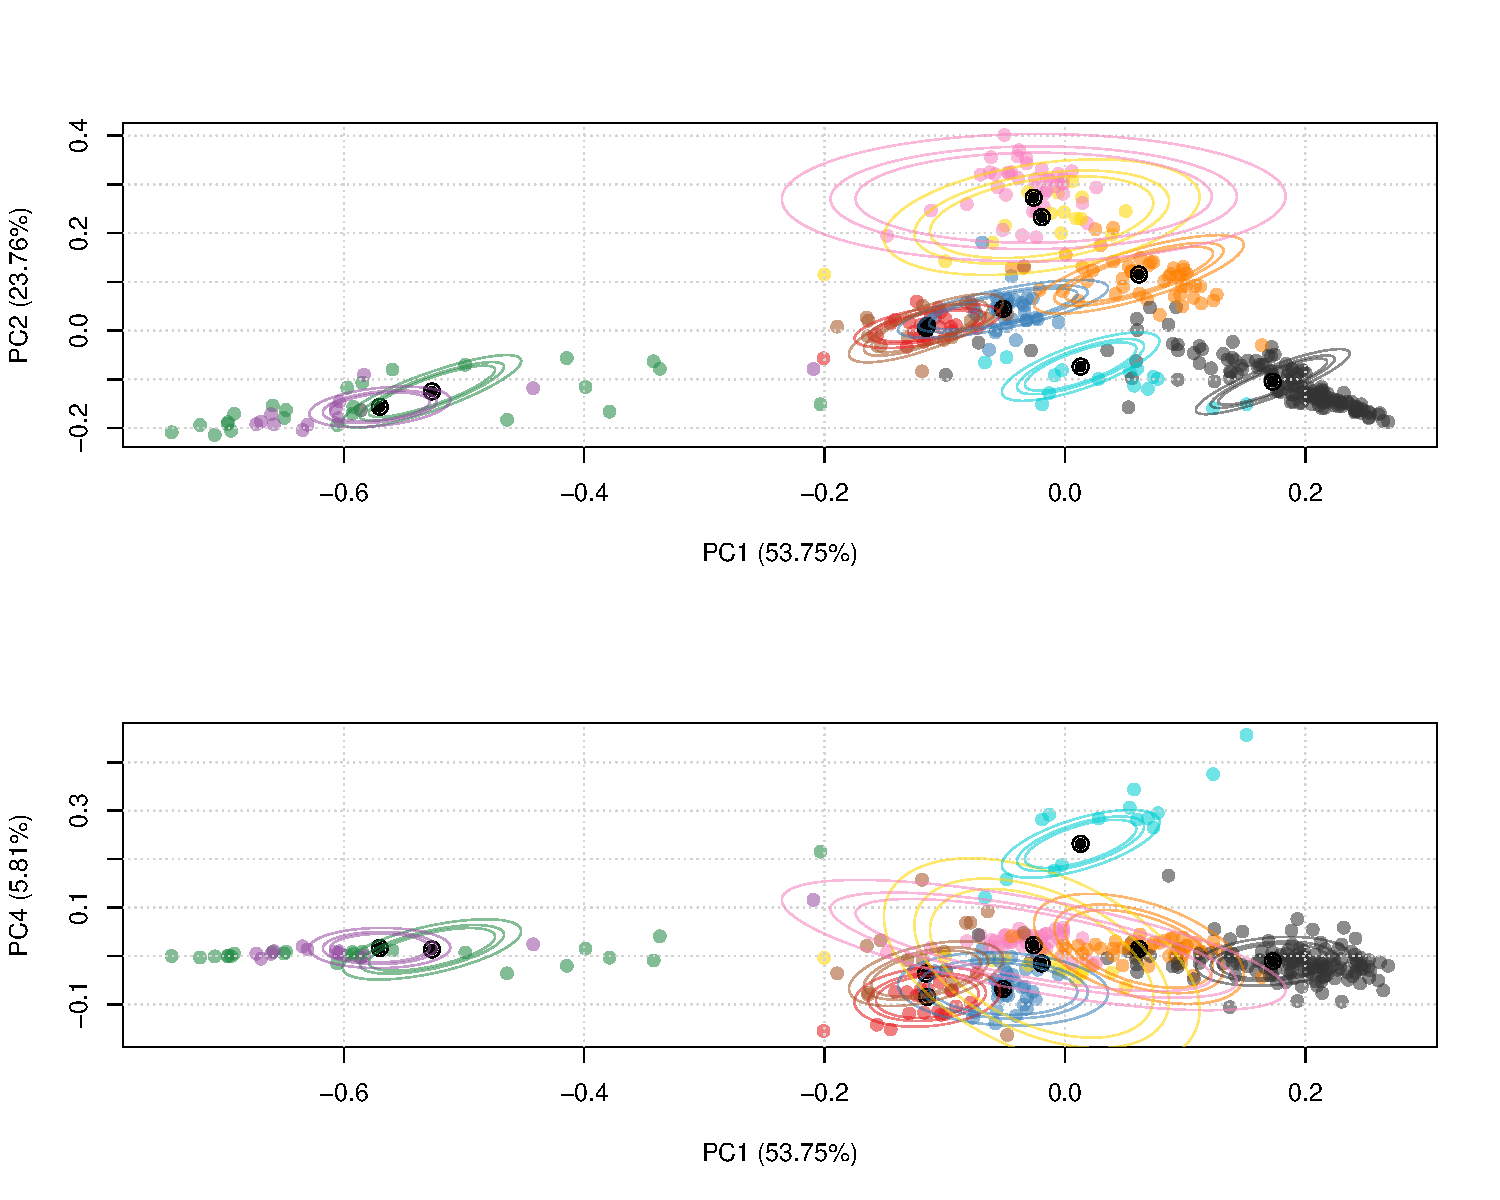
\includegraphics[width=1\linewidth]{F1000TAGMworkflow_rev1_files/figure-latex/e14ellipse-1} \caption{PCA plot with probability ellipses along PC 1 and 2 (left) and PC 1 and 4 (right). The ellipses show the component-conditional densities obtained from the fitted model evaluated at $ heta_{  ext{MAP}}$}\label{fig:e14ellipse}
\end{figure}

\hypertarget{the-expectation-maximisation-algorithm}{%
\subsection{The expectation-maximisation
algorithm}\label{the-expectation-maximisation-algorithm}}

The EM algorithm is iterative; that is, the algorithm iterates between
an expectation step and a maximisation step until the value of the
log-posterior does not change (Dempster, Laird, and Rubin 1977). This
fact can be used to assess the convergence of the EM algorithm. The
value of the log-posterior at each iteration can be accessed with the
\texttt{logPosteriors} function on the \texttt{MAPParams} object. The
code chunk below plots the log posterior at each iteration and we see on
figure @ref(fig:mapconverge) the algorithm rapidly plateaus and so we
have achieved convergence. If convergence has not been reached during
this time, we suggest to increase the number of iterations by changing
the parameter \texttt{numIter} in the \texttt{tagmMapTrain} method. In
practice, it is not unexpected to observe small fluctuations due to
numerical errors and this should not concern users.

\begin{Shaded}
\begin{Highlighting}[]
\KeywordTok{plot}\NormalTok{(}\KeywordTok{logPosteriors}\NormalTok{(mappars), }\DataTypeTok{type =} \StringTok{"b"}\NormalTok{, }\DataTypeTok{col =} \StringTok{"blue"}\NormalTok{,}
     \DataTypeTok{cex =} \FloatTok{0.3}\NormalTok{, }\DataTypeTok{ylab =} \StringTok{"log-posterior"}\NormalTok{, }\DataTypeTok{xlab =} \StringTok{"iteration"}\NormalTok{)}
\end{Highlighting}
\end{Shaded}

\begin{figure}
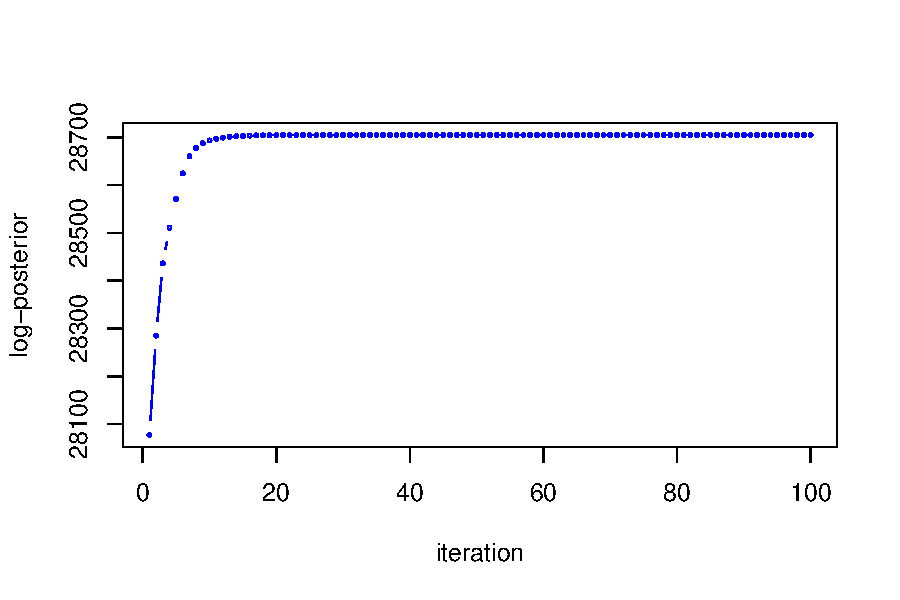
\includegraphics[width=0.8\linewidth]{F1000TAGMworkflow_rev1_files/figure-latex/mapconverge-1} \caption{Log-posterior at each iteration of the EM algorithm demonstrating convergence.}\label{fig:mapconverge}
\end{figure}

The code chunk below uses the \texttt{mappars} object generated above,
along with the \texttt{E14RG2aR} dataset, to classify the proteins of
unknown localisation using \texttt{tagmPredict} function. The results of
running \texttt{tagmPredict} are appended to the \texttt{fData} columns
of the \texttt{MSnSet}.

\begin{Shaded}
\begin{Highlighting}[]
\NormalTok{E14TG2aR <-}\StringTok{ }\KeywordTok{tagmPredict}\NormalTok{(E14TG2aR, mappars, }\DataTypeTok{probJoint =} \OtherTok{TRUE}\NormalTok{) }\CommentTok{# Predict protein localisation}
\end{Highlighting}
\end{Shaded}

The new feature variables that are generated are:

\begin{itemize}
\tightlist
\item
  \texttt{tagm.map.allocation}: the TAGM MAP predictions for the most
  probable protein sub-cellular allocation.
\end{itemize}

\begin{Shaded}
\begin{Highlighting}[]
\KeywordTok{table}\NormalTok{(}\KeywordTok{fData}\NormalTok{(E14TG2aR)}\OperatorTok{$}\NormalTok{tagm.map.allocation)}
\end{Highlighting}
\end{Shaded}

\begin{verbatim}
## 
##          40S Ribosome          60S Ribosome               Cytosol 
##                    34                    85                   328 
## Endoplasmic reticulum              Lysosome         Mitochondrion 
##                   284                   147                   341 
##   Nucleus - Chromatin   Nucleus - Nucleolus       Plasma membrane 
##                   143                   322                   326 
##            Proteasome 
##                    21
\end{verbatim}

\begin{itemize}
\tightlist
\item
  \texttt{tagm.map.probability}: the posterior probability for the
  protein sub-cellular allocations.
\end{itemize}

\begin{Shaded}
\begin{Highlighting}[]
\KeywordTok{summary}\NormalTok{(}\KeywordTok{fData}\NormalTok{(E14TG2aR)}\OperatorTok{$}\NormalTok{tagm.map.probability)}
\end{Highlighting}
\end{Shaded}

\begin{verbatim}
##    Min. 1st Qu.  Median    Mean 3rd Qu.    Max. 
## 0.00000 0.06963 0.93943 0.63829 0.99934 1.00000
\end{verbatim}

\begin{itemize}
\tightlist
\item
  \texttt{tagm.map.outlier}: the posterior probability for that protein
  to belong to the outlier component rather than any annotated
  component.
\end{itemize}

\begin{Shaded}
\begin{Highlighting}[]
\KeywordTok{summary}\NormalTok{(}\KeywordTok{fData}\NormalTok{(E14TG2aR)}\OperatorTok{$}\NormalTok{tagm.map.outlier)}
\end{Highlighting}
\end{Shaded}

\begin{verbatim}
##      Min.   1st Qu.    Median      Mean   3rd Qu.      Max. 
## 0.0000000 0.0002363 0.0305487 0.3452624 0.9249810 1.0000000
\end{verbatim}

We can visualise the results by scaling the pointer according the
posterior localisation probabilities. To do this we extract the MAP
localisation probabilities from the feature columns of the the
\texttt{MSnSet} and pass these to the \texttt{plot2D} function (figure
@ref(fig:mappca)).

\begin{Shaded}
\begin{Highlighting}[]
\NormalTok{ptsze <-}\StringTok{ }\KeywordTok{fData}\NormalTok{(E14TG2aR)}\OperatorTok{$}\NormalTok{tagm.map.probability }\CommentTok{# Scale pointer size}
\KeywordTok{plot2D}\NormalTok{(E14TG2aR, }\DataTypeTok{fcol =} \StringTok{"tagm.map.allocation"}\NormalTok{, }\DataTypeTok{cex =}\NormalTok{ ptsze)}
\KeywordTok{addLegend}\NormalTok{(E14TG2aR, }\DataTypeTok{where =} \StringTok{"topleft"}\NormalTok{, }\DataTypeTok{cex =} \FloatTok{0.6}\NormalTok{, }\DataTypeTok{fcol =} \StringTok{"tagm.map.allocation"}\NormalTok{)}
\end{Highlighting}
\end{Shaded}

\begin{figure}
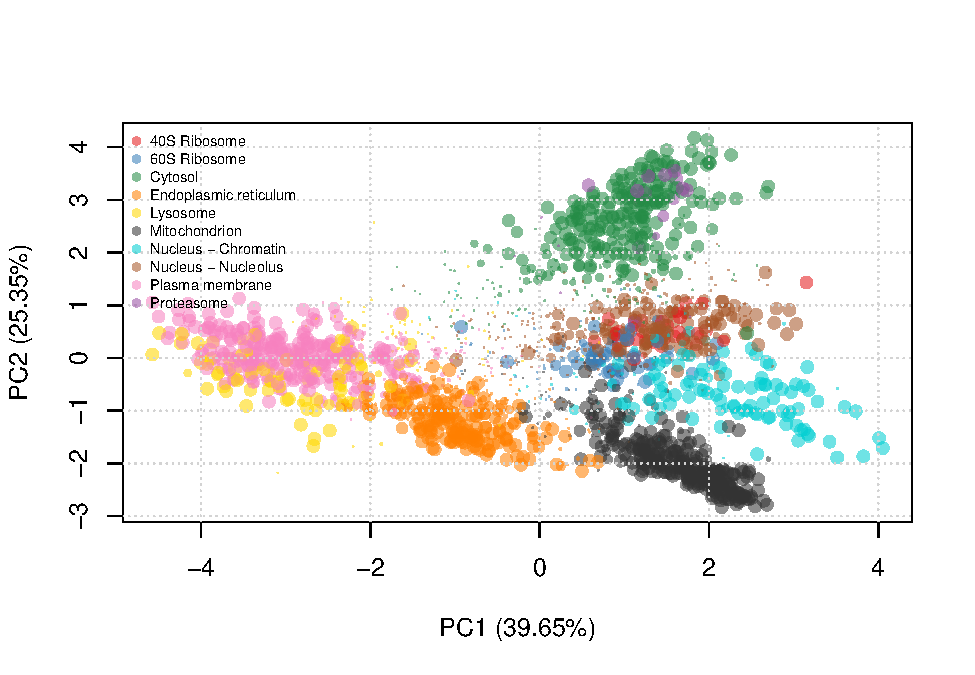
\includegraphics[width=0.7\linewidth]{F1000TAGMworkflow_rev1_files/figure-latex/mappca-1} \caption{TAGM MAP allocations, where the pointer is scaled according to the localisation probability and coloured according to the most probable subcellular niche.}\label{fig:mappca}
\end{figure}

The TAGM MAP method is easy to use and it is simple to check
convergence, however it is limited in that it can only provide point
estimates of the posterior localisation distributions. To obtain the
full posterior distributions and therefore a rich analysis of the data,
we use Markov-Chain Monte-Carlo methods. In our particular case, we use
a \emph{collapsed Gibbs sampler} (Smith and Roberts 1993).

\hypertarget{methods-tagm-mcmc-a-brief-overview}{%
\section{\texorpdfstring{Methods: \emph{TAGM MCMC} a brief
overview}{Methods: TAGM MCMC a brief overview}}\label{methods-tagm-mcmc-a-brief-overview}}

The TAGM MCMC method allows a fully Bayesian analysis of spatial
proteomics datasets. It employs a collapsed Gibbs sampler to sample from
the posterior distribution of localisation probablities, providing a
rich analysis of the data. This section demonstrates the advantage of
taking a Bayesian approach and the biological information that can be
extracted from this analysis.

For those unfamiliar with Bayesian methodology, some of the key ideas
for a more complete understanding are as follows. Firstly, MCMC based
inference contrasts with MAP based inference in that it \textit{samples}
from the posterior distribution of localisation probabilities. Hence, we
do not just have a single estimate for each quantity but a distribution
of estimates. MCMC methods are a large class of algorithms used to
sample from a probability distribution, in our case the posterior
distribution of the parameters (Gilks, Richardson, and Spiegelhalter
1995). Once we have sampled from the posterior distribution, we can
estimate the mean of the posterior distribution by simply taking the
mean of the samples. In a similar fashion, we can obtain estimates of
other summaries of the posterior distribution.

A schematic of MCMC sampling is provided in figure @ref(fig:mcmcCartoon)
to aid understanding. Proteins, coloured blue, are visualised along two
variables of the data. Probability ellipses representing contours of a
probability distribution matching the distribution of the proteins are
overlaid. We now wish to obtain samples from this distribution. The MCMC
algorithm is initialised with a starting location, then at each
iteration a new value is proposed. These proposed values are either
accepted or rejected (according to a carefully computed acceptance
probability) and over many iterations the algorithm converges and
produces samples from the desired distribution. Samples from this
distribution are coloured in red in the schematic figure. A large
portion of the earlier samples may not reflect the true distribution,
because the MCMC sampler has yet to converge. These early samples are
usually discarded and this is referred to as burn-in. The next state of
the algorithm depends on its current state and this leads to
auto-correlation in the samples. To suppress this auto-correlation, we
only retain every \(r^{th}\) sample. This is known as thinning. The
details of burn-in and thinning are further explained in later sections.

\begin{figure}
\centering
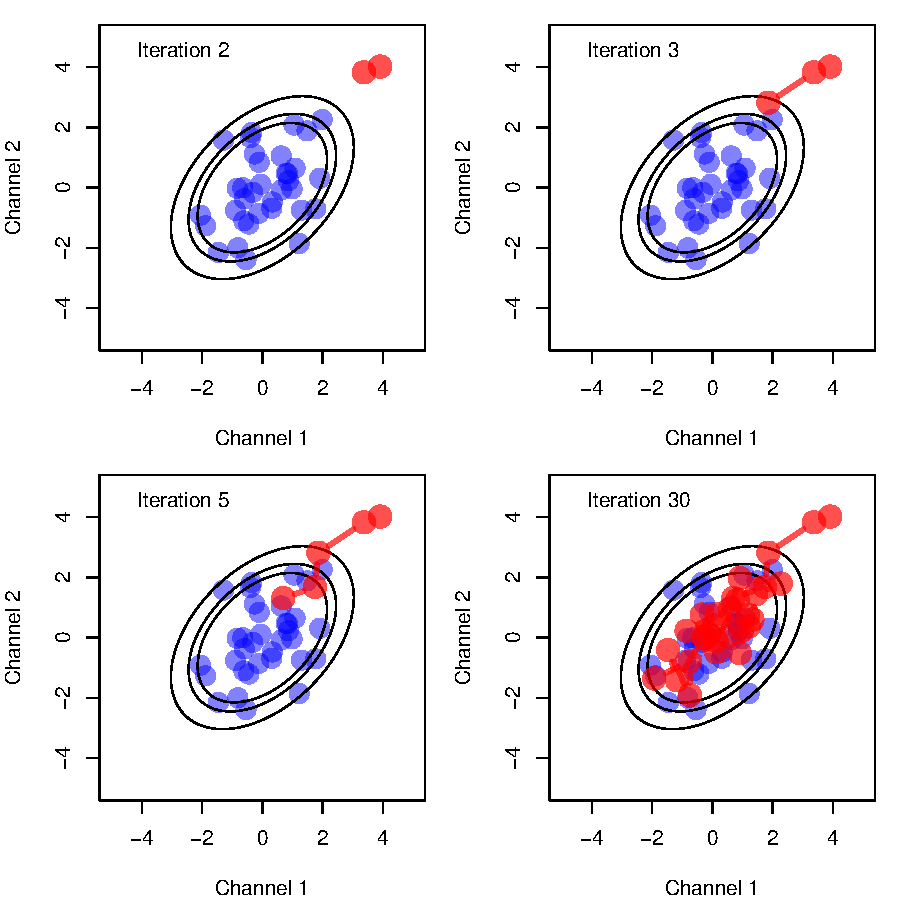
\includegraphics{F1000TAGMworkflow_rev1_files/figure-latex/mcmcCartoon-1.pdf}
\caption{A schematic figure of MCMC sampling. Proteins are coloured in
blue and probability ellipses are overlaid representing contours of a
probability distribution matching the distribution of the proteins. MCMC
samples from this distribution are then coloured in red.}
\end{figure}

The TAGM MCMC method is computationally intensive and requires at least
modest processing power. Leaving the MCMC algorithm to run overnight on
a modern desktop is usually sufficient, however this, of course, depends
on the particular dataset being analysed. For guidance: it should not be
expected that the analysis will finish in just a couple of hours on a
medium specification laptop, for example.

To demonstrate the class structure and expected outputs of the TAGM MCMC
method, we run a brief analysis on a subset (400 randomly chosen
proteins) of the \texttt{tan2009r1} dataset from the
\texttt{pRolocdata}, purely for illustration. This is to provide a bare
bones analysis of these data without being held back by computational
requirements. We perform a complete demonstration and provide precise
details of the analysis of the stem cell dataset considered above in the
next section.

\begin{Shaded}
\begin{Highlighting}[]
\KeywordTok{set.seed}\NormalTok{(}\DecValTok{1}\NormalTok{)}
\KeywordTok{data}\NormalTok{(tan2009r1)}
\NormalTok{tan2009r1 <-}\StringTok{ }\NormalTok{tan2009r1[}\KeywordTok{sample}\NormalTok{(}\KeywordTok{nrow}\NormalTok{(tan2009r1), }\DecValTok{400}\NormalTok{), ]}
\end{Highlighting}
\end{Shaded}

The first step is to run a few MCMC chains (below we use only 2 chains)
for a few iterations (we specify 3 iterations in the below code, but
typically we would suggest in the order of tens of thousands; see for
example the algorithms default settings by typing
\texttt{?tagmMcmcTrain}) using the \texttt{tagmMcmcTrain} function. This
function will generate a object of class \texttt{MCMCParams}.

\begin{Shaded}
\begin{Highlighting}[]
\NormalTok{p <-}\StringTok{ }\KeywordTok{tagmMcmcTrain}\NormalTok{(}\DataTypeTok{object =}\NormalTok{ tan2009r1, }\DataTypeTok{numIter =} \DecValTok{3}\NormalTok{,}
                   \DataTypeTok{burnin =} \DecValTok{1}\NormalTok{, }\DataTypeTok{thin =} \DecValTok{1}\NormalTok{, }\DataTypeTok{numChains =} \DecValTok{2}\NormalTok{)}
\NormalTok{p}
\end{Highlighting}
\end{Shaded}

\begin{verbatim}
## Object of class "MCMCParams"
## Method: TAGM.MCMC 
## Number of chains: 2
\end{verbatim}

Information for each MCMC chain is contained within the chains slot. If
needed, this information can be accessed manually. The function
\texttt{tagmMcmcProcess} processes the \texttt{MCMCParams} object and
populates the summary slot.

\begin{Shaded}
\begin{Highlighting}[]
\NormalTok{p <-}\StringTok{ }\KeywordTok{tagmMcmcProcess}\NormalTok{(p)}
\NormalTok{p}
\end{Highlighting}
\end{Shaded}

\begin{verbatim}
## Object of class "MCMCParams"
## Method: TAGM.MCMC 
## Number of chains: 2 
## Summary available
\end{verbatim}

The summary slot has now been populated to include basic summaries of
the MCMC chains, such as organelle allocations and localisation
probabilities. Protein information can be appended to the feature
columns of the \texttt{MSnSet} by using the \texttt{tagmPredict}
function, which extracts the required information from the summary slot
of the \texttt{MCMCParams} object.

\begin{Shaded}
\begin{Highlighting}[]
\NormalTok{res <-}\StringTok{ }\KeywordTok{tagmPredict}\NormalTok{(}\DataTypeTok{object =}\NormalTok{ tan2009r1, }\DataTypeTok{params =}\NormalTok{ p)}
\end{Highlighting}
\end{Shaded}

We can now access new variables:

\begin{itemize}
\tightlist
\item
  \texttt{tagm.mcmc.allocation}: the TAGM MCMC prediction for the most
  likely protein sub-cellular annotation.
\end{itemize}

\begin{Shaded}
\begin{Highlighting}[]
\KeywordTok{table}\NormalTok{(}\KeywordTok{fData}\NormalTok{(res)}\OperatorTok{$}\NormalTok{tagm.mcmc.allocation)}
\end{Highlighting}
\end{Shaded}

\begin{verbatim}
## 
##  Cytoskeleton            ER         Golgi      Lysosome mitochondrion 
##            11            98            24             9            39 
##       Nucleus    Peroxisome            PM    Proteasome  Ribosome 40S 
##            26             3           102            29            30 
##  Ribosome 60S 
##            29
\end{verbatim}

\begin{itemize}
\tightlist
\item
  \texttt{tagm.mcmc.probability}: the mean posterior probability for the
  protein sub-cellular allocations.
\end{itemize}

\begin{Shaded}
\begin{Highlighting}[]
\KeywordTok{summary}\NormalTok{(}\KeywordTok{fData}\NormalTok{(res)}\OperatorTok{$}\NormalTok{tagm.mcmc.probability)}
\end{Highlighting}
\end{Shaded}

\begin{verbatim}
##    Min. 1st Qu.  Median    Mean 3rd Qu.    Max. 
##  0.3267  0.8692  0.9881  0.9038  1.0000  1.0000
\end{verbatim}

We can also access other useful summaries of the MCMC methods:

\begin{itemize}
\item
  \texttt{tagm.mcmc.outlier} the posterior probability for the protein
  to belong to the outlier component.
\item
  \texttt{tagm.mcmc.probability.lowerquantile} and
  \texttt{tagm.mcmc.probability.upperquantile} are the lower and upper
  boundaries to the equi-tailed 95\% credible interval of
  \texttt{tagm.mcmc.probability}.
\item
  \texttt{tagm.mcmc.mean.shannon} a Monte-Carlo averaged Shannon
  entropy, which is a measure of uncertainty in the allocations.
\end{itemize}

\hypertarget{methods-tagm-mcmc-the-details}{%
\section{\texorpdfstring{Methods: \emph{TAGM MCMC} the
details}{Methods: TAGM MCMC the details}}\label{methods-tagm-mcmc-the-details}}

This section explains how to manually manipulate the MCMC output of the
TAGM model. In the code chunk below, we load a pre-computed TAGM MCMC
model. The data file \texttt{e14tagm.rda} is available online\footnote{\url{https://drive.google.com/open?id=1zozntDhE6YZ-q8wjtQ-lxZ66EEszOGYi}}
and is not directly loaded into this package due to its size. The file
itself if around 500mb, which is too large to directly load into a
package.

\begin{Shaded}
\begin{Highlighting}[]
\KeywordTok{load}\NormalTok{(}\StringTok{"e14Tagm.rda"}\NormalTok{)}
\end{Highlighting}
\end{Shaded}

The following code, which is not evaluated dynamically, was used to
produce the \texttt{tagmE14} \texttt{MCMCParams} object. We run the MCMC
algorithm for 20,000 iterations with 10,000 iterations discarded for
burn-in. We then thin the chain by 20. We ran 6 chains in parallel and
so we obtain 500 samples for each of the 6 chains, totalling 3,000
samples. The resulting file is assumed to be in our working directory.

\begin{Shaded}
\begin{Highlighting}[]
\NormalTok{e14Tagm <-}\StringTok{ }\KeywordTok{tagmMcmcTrain}\NormalTok{(E14TG2aR,}
                         \DataTypeTok{numIter =} \DecValTok{20000}\NormalTok{,}
                         \DataTypeTok{burnin =} \DecValTok{10000}\NormalTok{,}
                         \DataTypeTok{thin =} \DecValTok{20}\NormalTok{,}
                         \DataTypeTok{numChains =} \DecValTok{6}\NormalTok{)}
\end{Highlighting}
\end{Shaded}

Manually inspecting the object, we see that it is a \texttt{MCMCParams}
object with 6 chains.

\begin{Shaded}
\begin{Highlighting}[]
\NormalTok{e14Tagm}
\end{Highlighting}
\end{Shaded}

\begin{verbatim}
## Object of class "MCMCParams"
## Method: TAGM.MCMC 
## Number of chains: 6
\end{verbatim}

\hypertarget{data-exploration-and-convergence-diagnostics}{%
\subsection{Data exploration and convergence
diagnostics}\label{data-exploration-and-convergence-diagnostics}}

Assessing whether or not an MCMC algorithm has converged is challenging.
Assessing and diagnosing convergence is an active area of research and
throughout the 1990s many approaches were proposed (Geweke 1992; Gelman
and Rubin 1992; Roberts and Smith 1994; Brooks and Gelman 1998) and
these discussions have been refined in recent years (see (Vats and
Knudson 2018), (Vehtari et al. 2019)). We provide a more detailed
exploration of this issue, but readers should bear in mind that the
methods provided below are diagnostics and cannot guarantee convergence.
We direct readers to several important works in the literature
discussing the assessment of convergence. Users that do not assess
convergence and base their downstream analysis on unconverged chains are
likely to obtain poor quality results.

We first assess convergence using a parallel chains approach. We find
producing multiple chains is benificial not only for computational
advantages but also for analysis of convergence of our chains. As with
other authors, we suggest a minimum of 4 chains (Vehtari et al. 2019).
This is the default setting in the software. However, in this workflow
we run \(6\) chains to highlight some challenges.

\begin{Shaded}
\begin{Highlighting}[]
\CommentTok{## Get number of chains}
\NormalTok{nChains <-}\StringTok{ }\KeywordTok{length}\NormalTok{(e14Tagm)}
\NormalTok{nChains}
\end{Highlighting}
\end{Shaded}

\begin{verbatim}
## [1] 6
\end{verbatim}

The following code chunks set up a manual convergence diagnostic check.
We make use of objects and methods in the package
\emph{\href{https://CRAN.R-project.org/package=coda}{coda}} to perform
this analysis (Plummer et al. 2006). Our function below automatically
coerces our objects into
\emph{\href{https://CRAN.R-project.org/package=coda}{coda}} for ease of
analysis. We first calculate the total number of outliers at each
iteration of each chain and, if the algorithm has converged, this number
should be the same (or very similar) across all 6 chains.

\begin{Shaded}
\begin{Highlighting}[]
\CommentTok{## Convergence diagnostic to see if we need to discard any}
\CommentTok{## iterations or entire chains: compute the number of outliers for}
\CommentTok{## each iteration for each chain}
\NormalTok{out <-}\StringTok{ }\KeywordTok{mcmc_get_outliers}\NormalTok{(e14Tagm)}
\end{Highlighting}
\end{Shaded}

We can observe this from the trace plots and histograms for each MCMC
chain (figure @ref(fig:mcmctraceHidden)). Unconverged chains should be
discarded from downstream analysis.

\begin{figure}
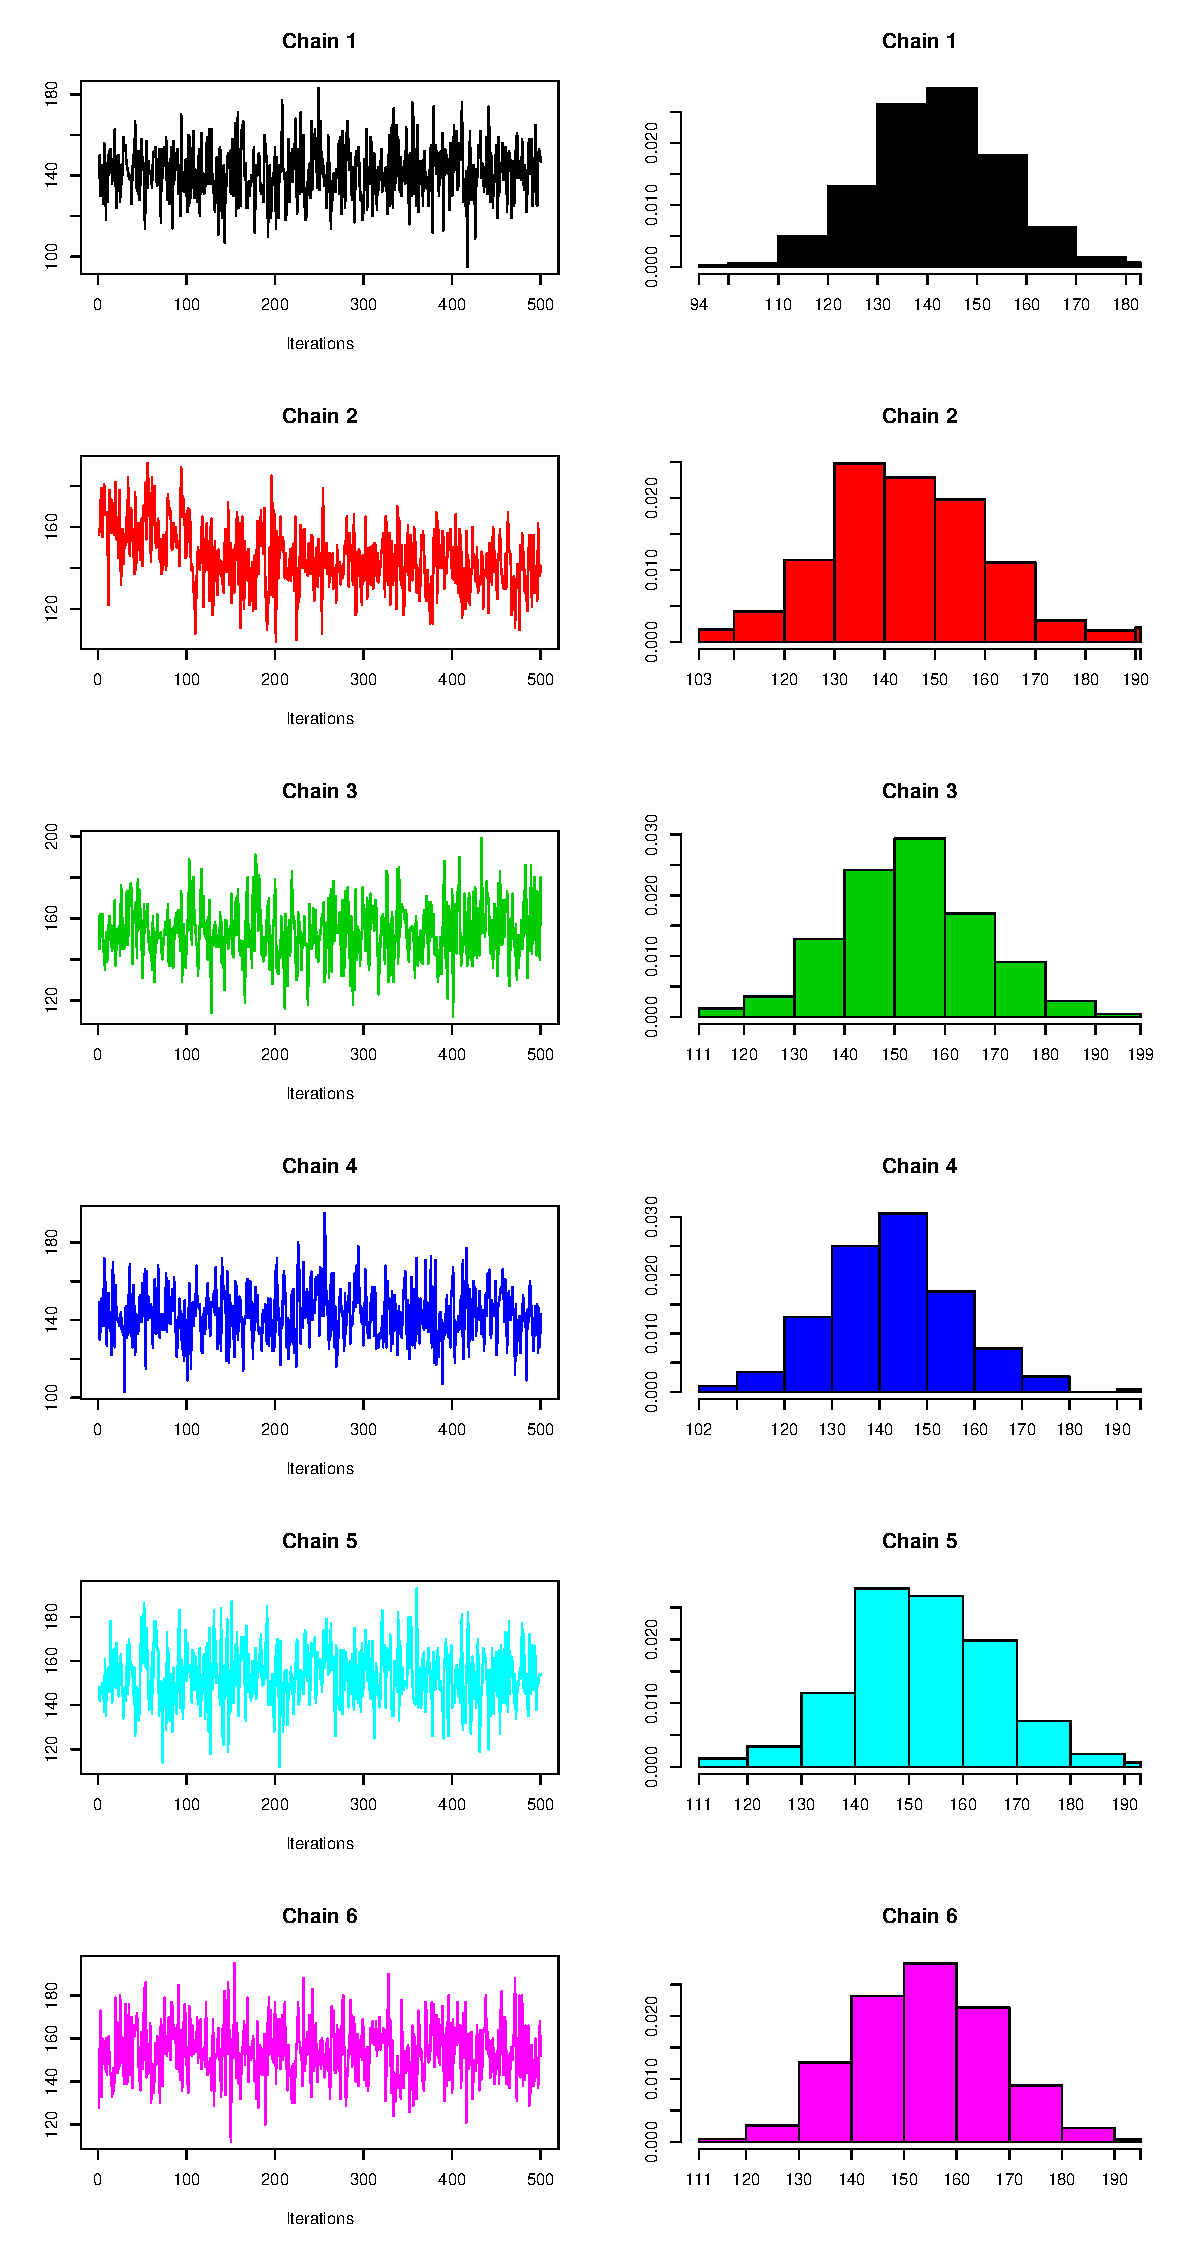
\includegraphics[width=0.7\linewidth]{F1000TAGMworkflow_rev1_files/figure-latex/mcmctraceHidden-1} \caption{Trace (left) and density (right) of the 6 MCMC chains. 500 iterations were subsampled from the MCMC chains of 20,000 iterations}\label{fig:mcmctraceHidden}
\end{figure}

\begin{Shaded}
\begin{Highlighting}[]
\CommentTok{## Using coda S3 objects to produce trace plots and histograms}
\ControlFlowTok{for}\NormalTok{ (i }\ControlFlowTok{in} \KeywordTok{seq_len}\NormalTok{(nChains))}
    \KeywordTok{plot}\NormalTok{(out[[i]], }\DataTypeTok{main =} \KeywordTok{paste}\NormalTok{(}\StringTok{"Chain"}\NormalTok{, i), }\DataTypeTok{auto.layout =} \OtherTok{FALSE}\NormalTok{, }\DataTypeTok{col =}\NormalTok{ i)}
\end{Highlighting}
\end{Shaded}

Chains 3, 5 and 6 are centred around an average of 153, with rapid back
and forth oscillations. Chain 2 should be immediately discarded, since
it has a large jump in the chain with clearly skewed histogram. The
other two chains oscillate differently with contrasting quantiles to the
3 chains (3, 5 and 6) that agree with one another, suggesting these
chains have yet to converge. We can use the
\emph{\href{https://CRAN.R-project.org/package=coda}{coda}} package to
produce summaries of our chains. Here is the \texttt{coda} summary for
the third chain.

\begin{Shaded}
\begin{Highlighting}[]
\CommentTok{## Chains average around 153 outliers}
\KeywordTok{summary}\NormalTok{(out[[}\DecValTok{3}\NormalTok{]])}
\end{Highlighting}
\end{Shaded}

\begin{verbatim}
## 
## Iterations = 1:500
## Thinning interval = 1 
## Number of chains = 1 
## Sample size per chain = 500 
## 
## 1. Empirical mean and standard deviation for each variable,
##    plus standard error of the mean:
## 
##           Mean             SD       Naive SE Time-series SE 
##       153.4520        14.0771         0.6295         0.6820 
## 
## 2. Quantiles for each variable:
## 
##  2.5%   25%   50%   75% 97.5% 
##   127   144   153   162   183
\end{verbatim}

\hypertarget{applying-the-gelman-diagnostic}{%
\subsubsection{Applying the Gelman
diagnostic}\label{applying-the-gelman-diagnostic}}

So far, our analysis appears promising. Three of our chains are centred
around an average of 153 outliers and there is no observed monotonicity
in our output. However, for a more rigorous and unbiased analysis of
convergence we can calculate the Gelman diagnostic using the
\emph{\href{https://CRAN.R-project.org/package=coda}{coda}} package
(Gelman and Rubin 1992; Brooks and Gelman 1998). This statistic is often
referred to as \(\hat{R}\) or the potential scale reduction factor. The
idea of the Gelman diagnostics is to compare the inter and intra chain
variances. The ratio of these quantities should be close to one. A more
detailed and in depth discussion can be found in the references. The
\emph{\href{https://CRAN.R-project.org/package=coda}{coda}} package also
reports the \(95\%\) upper confidence interval of the \(\hat{R}\)
statistic. In this case, our samples are approximately normally
distributed (see histograms on the right in figure
@ref(fig:mcmctraceHidden)). The
\emph{\href{https://CRAN.R-project.org/package=coda}{coda}} package
allows for transformations to improve normality of the data, and in some
cases we set the \texttt{transform} argument to apply log
transformation. Gelman and Rubin (1992) suggest that chains with
\(\hat{R}\) value of less than 1.2 are likely to have converged, though
recent literature suggests considerably smaller values and a thredhold
of \(1.01\) is likely to lead to more stable and reliable results (Vats
and Knudson 2018; Vehtari et al. 2019).

\begin{Shaded}
\begin{Highlighting}[]
\KeywordTok{gelman.diag}\NormalTok{(out, }\DataTypeTok{transform =} \OtherTok{FALSE}\NormalTok{)}
\end{Highlighting}
\end{Shaded}

\begin{verbatim}
## Potential scale reduction factors:
## 
##      Point est. Upper C.I.
## [1,]       1.14       1.32
\end{verbatim}

\begin{Shaded}
\begin{Highlighting}[]
\KeywordTok{gelman.diag}\NormalTok{(out[}\KeywordTok{c}\NormalTok{(}\DecValTok{1}\NormalTok{, }\DecValTok{3}\NormalTok{, }\DecValTok{4}\NormalTok{, }\DecValTok{5}\NormalTok{, }\DecValTok{6}\NormalTok{)], }\DataTypeTok{transform =} \OtherTok{FALSE}\NormalTok{)}
\end{Highlighting}
\end{Shaded}

\begin{verbatim}
## Potential scale reduction factors:
## 
##      Point est. Upper C.I.
## [1,]       1.13       1.31
\end{verbatim}

\begin{Shaded}
\begin{Highlighting}[]
\KeywordTok{gelman.diag}\NormalTok{(out[}\KeywordTok{c}\NormalTok{(}\DecValTok{3}\NormalTok{, }\DecValTok{5}\NormalTok{, }\DecValTok{6}\NormalTok{)], }\DataTypeTok{transform =} \OtherTok{FALSE}\NormalTok{)}
\end{Highlighting}
\end{Shaded}

\begin{verbatim}
## Potential scale reduction factors:
## 
##      Point est. Upper C.I.
## [1,]          1       1.01
\end{verbatim}

In all cases, we see that the Gelman diagnostic for convergence is
\textless{} 1.2, but only in the final case is it \textless{} 1.01.
However, the upper confidence interval is 1.32 when all chains are used;
1.31 when chain 2 is removed and when chains 1, 2 and 4 are removed the
upper confidence interval is 1.01 indicating that the MCMC algorithm for
chains 3, 5 and 6 might have converged.

We can also look at the Gelman diagnostics statistics for groups or
pairs of chains. The first line below computes the Gelman diagnostic
across the first three chains, whereas the second calculates the
diagnostic between chain 3 and chain 5.

\begin{Shaded}
\begin{Highlighting}[]
\KeywordTok{gelman.diag}\NormalTok{(out[}\DecValTok{1}\OperatorTok{:}\DecValTok{3}\NormalTok{], }\DataTypeTok{transform =} \OtherTok{FALSE}\NormalTok{) }\CommentTok{# the upper C.I is 1.62}
\end{Highlighting}
\end{Shaded}

\begin{verbatim}
## Potential scale reduction factors:
## 
##      Point est. Upper C.I.
## [1,]       1.22       1.62
\end{verbatim}

\begin{Shaded}
\begin{Highlighting}[]
\KeywordTok{gelman.diag}\NormalTok{(out[}\KeywordTok{c}\NormalTok{(}\DecValTok{3}\NormalTok{, }\DecValTok{5}\NormalTok{)], }\DataTypeTok{transform =} \OtherTok{TRUE}\NormalTok{) }\CommentTok{# the upper C.I is 1.01}
\end{Highlighting}
\end{Shaded}

\begin{verbatim}
## Potential scale reduction factors:
## 
##      Point est. Upper C.I.
## [1,]       1.01       1.01
\end{verbatim}

To assess another summary statistic, we can look at the mean component
allocation at each iteration of the MCMC algorithm and as before we
produce trace plots of this quantity (figure
@ref(fig:mcmctrace2hidden)).

\begin{Shaded}
\begin{Highlighting}[]
\NormalTok{meanAlloc <-}\StringTok{ }\KeywordTok{mcmc_get_meanComponent}\NormalTok{(e14Tagm)}
\end{Highlighting}
\end{Shaded}

\begin{figure}
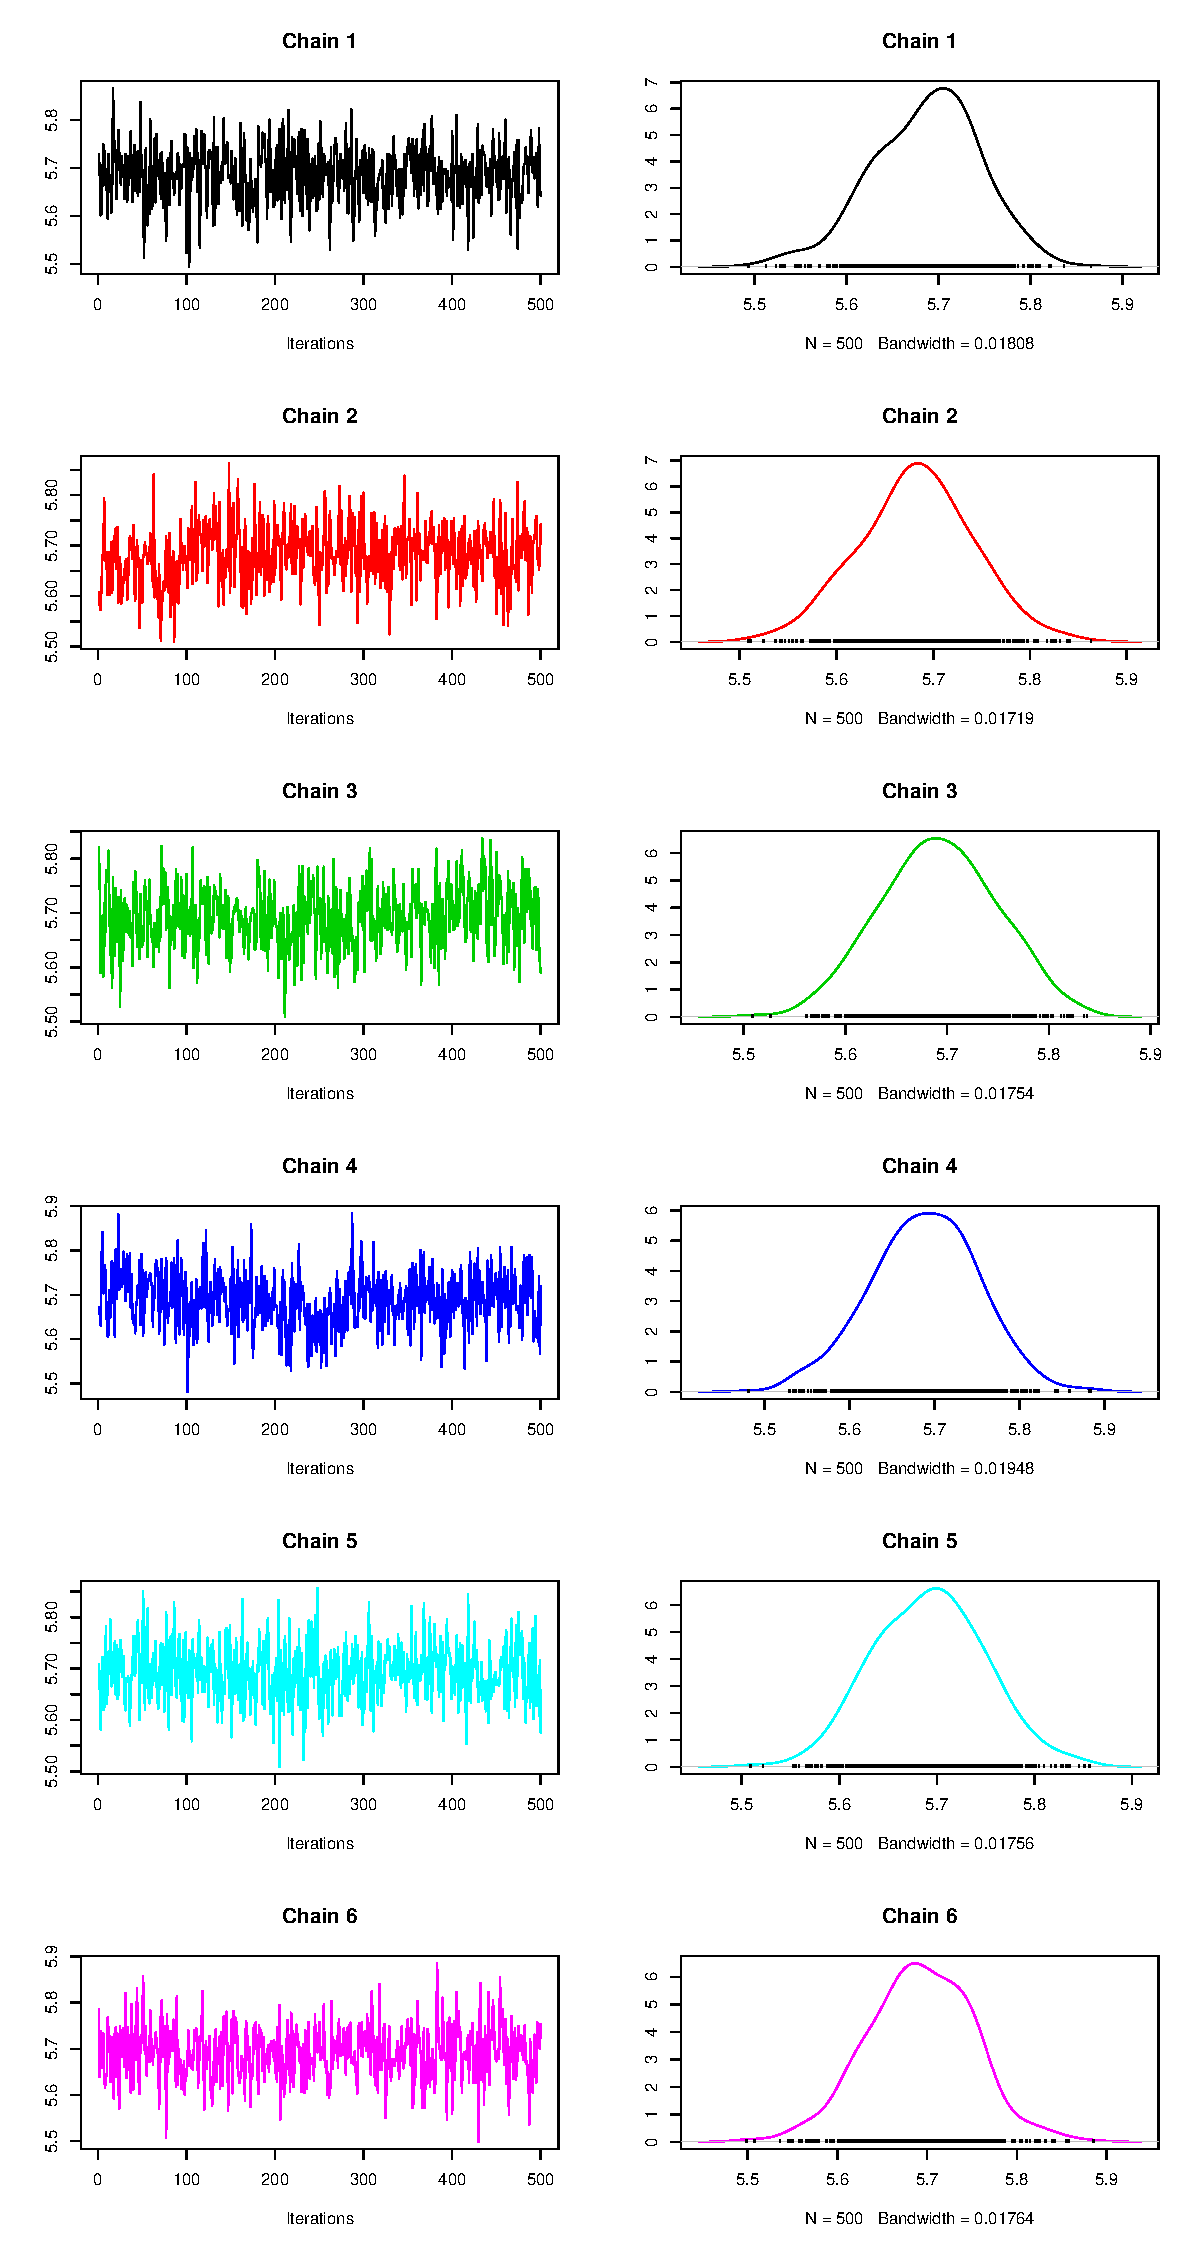
\includegraphics[width=0.7\linewidth]{F1000TAGMworkflow_rev1_files/figure-latex/mcmctrace2hidden-1} \caption{Trace (left) and density (right) of the mean component allocation of the 6 MCMC chains. 500 iterations were subsampled from the MCMC chains of 20,000 iterations.}\label{fig:mcmctrace2hidden}
\end{figure}

\begin{Shaded}
\begin{Highlighting}[]
\ControlFlowTok{for}\NormalTok{ (i }\ControlFlowTok{in} \KeywordTok{seq_len}\NormalTok{(nChains))}
    \KeywordTok{plot}\NormalTok{(meanAlloc[[i]], }\DataTypeTok{main =} \KeywordTok{paste}\NormalTok{(}\StringTok{"Chain"}\NormalTok{, i), }\DataTypeTok{auto.layout =} \OtherTok{FALSE}\NormalTok{, }\DataTypeTok{col =}\NormalTok{ i)}
\end{Highlighting}
\end{Shaded}

As before we can produce summaries of the data.

\begin{Shaded}
\begin{Highlighting}[]
\KeywordTok{summary}\NormalTok{(meanAlloc[[}\DecValTok{1}\NormalTok{]])}
\end{Highlighting}
\end{Shaded}

\begin{verbatim}
## 
## Iterations = 1:500
## Thinning interval = 1 
## Number of chains = 1 
## Sample size per chain = 500 
## 
## 1. Empirical mean and standard deviation for each variable,
##    plus standard error of the mean:
## 
##           Mean             SD       Naive SE Time-series SE 
##       5.686713       0.059112       0.002644       0.002644 
## 
## 2. Quantiles for each variable:
## 
##  2.5%   25%   50%   75% 97.5% 
## 5.552 5.646 5.692 5.728 5.795
\end{verbatim}

We can already observed that there are some slight differences between
these chains, which raises suspicion that some of the chains may not
have converged. For example each chain appears to be centred around 5.7,
but chains 2 and 4 have clear jumps in the their trace plots. To be more
precise, we note the jump that occurs are between iteration 100-150 in
chain 2 and between iteration 200-250 in chain 4. For a more
quantitative analysis, we again apply the Gelman diagnostics to these
summaries.

\begin{Shaded}
\begin{Highlighting}[]
\KeywordTok{gelman.diag}\NormalTok{(meanAlloc)}
\end{Highlighting}
\end{Shaded}

\begin{verbatim}
## Potential scale reduction factors:
## 
##      Point est. Upper C.I.
## [1,]          1       1.01
\end{verbatim}

The above values are close to 1 and so there are no significant
differences between the chains. As observed previously, chains 2 and 4
look quite different from the other chains and so we recalculate the
diagnostic excluding these chains. The computed Gelman diagnostic below
suggest that chains 3, 5 and 6 have converged and that we should discard
chains 1, 2 and 4 from further analysis.

\begin{Shaded}
\begin{Highlighting}[]
\KeywordTok{gelman.diag}\NormalTok{(meanAlloc[}\KeywordTok{c}\NormalTok{(}\DecValTok{3}\NormalTok{, }\DecValTok{5}\NormalTok{, }\DecValTok{6}\NormalTok{)])}
\end{Highlighting}
\end{Shaded}

\begin{verbatim}
## Potential scale reduction factors:
## 
##      Point est. Upper C.I.
## [1,]          1          1
\end{verbatim}

For a further check, we can look at the mean outlier probability at each
iteration of the MCMC algorithm and again computing the Gelman
diagnostics between chains 3, 5 and 6. An \(\hat{R}\) statistic of 1 is
indicative of convergence, since it is less than the recommended value
of 1.01.

\begin{Shaded}
\begin{Highlighting}[]
\NormalTok{meanoutProb <-}\StringTok{ }\KeywordTok{mcmc_get_meanoutliersProb}\NormalTok{(e14Tagm)}
\KeywordTok{gelman.diag}\NormalTok{(meanoutProb[}\KeywordTok{c}\NormalTok{(}\DecValTok{3}\NormalTok{, }\DecValTok{5}\NormalTok{, }\DecValTok{6}\NormalTok{)])}
\end{Highlighting}
\end{Shaded}

\begin{verbatim}
## Potential scale reduction factors:
## 
##      Point est. Upper C.I.
## [1,]          1       1.01
\end{verbatim}

\hypertarget{applying-the-geweke-diagnostic}{%
\subsubsection{Applying the Geweke
diagnostic}\label{applying-the-geweke-diagnostic}}

Along with the Gelman diagnostic, which uses parallel chains, we can
also apply a single chain analysis using the Geweke diagnostic (Geweke
1992). The Geweke diagnostic tests to see whether the mean calculated
from the first \(10\%\) of iterations is significantly different from
the mean calculated from the last \(50\%\) of iterations. If they are
significantly different, at say a level 0.01, then this is evidence that
particular chains have not converged. The following code chunk
calculates the Geweke diagnostic for each chain on the summarising
quantities we have previously computed.

\begin{Shaded}
\begin{Highlighting}[]
\KeywordTok{geweke_test}\NormalTok{(out)}
\end{Highlighting}
\end{Shaded}

\begin{verbatim}
##           chain 1      chain 2  chain 3    chain 4    chain 5    chain 6
## z.value 0.5749775 8.816632e+00 0.470203 -0.3204500 -0.6270787 -0.7328168
## p.value 0.5653065 1.179541e-18 0.638210  0.7486272  0.5306076  0.4636702
\end{verbatim}

\begin{Shaded}
\begin{Highlighting}[]
\KeywordTok{geweke_test}\NormalTok{(meanAlloc)}
\end{Highlighting}
\end{Shaded}

\begin{verbatim}
##           chain 1       chain 2    chain 3    chain 4   chain 5    chain 6
## z.value 1.1952967 -3.3737051063 -1.2232102 2.48951993 0.3605882 -0.1358850
## p.value 0.2319711  0.0007416377  0.2212503 0.01279157 0.7184073  0.8919122
\end{verbatim}

\begin{Shaded}
\begin{Highlighting}[]
\KeywordTok{geweke_test}\NormalTok{(meanoutProb)}
\end{Highlighting}
\end{Shaded}

\begin{verbatim}
##           chain 1      chain 2   chain 3    chain 4    chain 5     chain 6
## z.value 0.1785882 1.205500e+01 0.6189637 -0.5164987 -0.2141086 -0.02379004
## p.value 0.8582611 1.825379e-33 0.5359403  0.6055062  0.8304624  0.98102008
\end{verbatim}

The first test suggests chain 2 has not converged, since the p-value is
less than \(10^{-10}\) suggesting that the mean in the first \(10\%\) of
iterations is significantly different from those in the final \(50\%\).
Moreover, the second test and third tests also suggest that chain 2 has
not converged. Furthermore, for the second test chain 4 has a marginally
small p-value, providing further evidence that this chain is of low
quality. These convergence diagnostics are not limited to the quantities
we have computed here and further diagnostics can be performed on any
summary of the data.

An important question to consider is whether removing an early portion
of the chain might lead to an improvement of the convergence
diagnostics. This might be particularly relevant if a chain converges
some iterations after our orginally specified \texttt{burn-in}. For
example, let us take the second Geweke test above, which suggested
chains 2 and 4 had not converged and see if discarding the initial
\(10\%\) of the chain improves the statistic. The function below removes
\(50\) samples, known as \texttt{burn-in}, from the beginning of each
chain and the output shows that we now have \(450\) samples in each
chain. In practice, as \(2\) chains are sufficient for good posterior
estimates and convergence we could simply discard chains \(2\) and \(4\)
and proceed with downstream analysis with the remaining chains.

\begin{Shaded}
\begin{Highlighting}[]
\NormalTok{burn_e14Tagm <-}\StringTok{ }\KeywordTok{mcmc_burn_chains}\NormalTok{(e14Tagm, }\DecValTok{50}\NormalTok{)}
\KeywordTok{chains}\NormalTok{(burn_e14Tagm)}
\end{Highlighting}
\end{Shaded}

\begin{verbatim}
## Object of class "MCMCChains"
##  Number of chains: 6
\end{verbatim}

\begin{Shaded}
\begin{Highlighting}[]
\KeywordTok{chains}\NormalTok{(burn_e14Tagm)[[}\DecValTok{4}\NormalTok{]]}
\end{Highlighting}
\end{Shaded}

\begin{verbatim}
## Object of class "MCMCChain"
##  Number of components: 10 
##  Number of proteins: 1663 
##  Number of iterations: 450
\end{verbatim}

The following function recomputes the number of outliers in each chain
at each iteration of each Markov-chain.

\begin{Shaded}
\begin{Highlighting}[]
\NormalTok{out2 <-}\StringTok{ }\KeywordTok{mcmc_get_outliers}\NormalTok{(burn_e14Tagm)}
\end{Highlighting}
\end{Shaded}

The code chunk below computes the Geweke diagnostic for this new
truncated chain and demonstrates that chain 4 has an improved Geweke
diagnostic, whilst chain 2 does not. Thus, in practice, it maybe useful
to remove iterations from the beginning of the chain. However, as chain
4 did not pass the Gelman diagnostics we still discard it from
downstream analysis.

\begin{Shaded}
\begin{Highlighting}[]
\KeywordTok{geweke_test}\NormalTok{(out2)}
\end{Highlighting}
\end{Shaded}

\begin{verbatim}
##            chain 1      chain 2    chain 3   chain 4   chain 5   chain 6
## z.value -0.1455345 6.379618e+00 -1.6392215 0.3836940 0.1241201 0.6654703
## p.value  0.8842889 1.775298e-10  0.1011671 0.7012053 0.9012202 0.5057497
\end{verbatim}

In this section, we have highlighted that assessing convergence is an
essential part of Bayesian analysis. As well as the summaries considered
here, we recommend that users assess other posterior summaries of the
data. Since the best practices for assessing convergence also change
overtime, we also suggest searching the literature for current
consensus.

\hypertarget{processing-converged-chains}{%
\subsection{Processing converged
chains}\label{processing-converged-chains}}

Having made an assessment of convergence, we decide to discard chains
\(1,2\) and \(4\) from any further analysis. The code chunk below
removes these chains and creates a new object to store the converged
chains.

\begin{Shaded}
\begin{Highlighting}[]
\NormalTok{removeChain <-}\StringTok{ }\KeywordTok{c}\NormalTok{(}\DecValTok{1}\NormalTok{, }\DecValTok{2}\NormalTok{, }\DecValTok{4}\NormalTok{) }\CommentTok{# The chains to be removed}
\NormalTok{e14Tagm_converged <-}\StringTok{ }\NormalTok{e14Tagm[}\OperatorTok{-}\NormalTok{removeChain] }\CommentTok{# Create new object}
\end{Highlighting}
\end{Shaded}

The \texttt{MCMCParams} object can be large and therefore if we have a
large number of samples we may want to subsample our chain, known as
\emph{thinning}, to reduce the number of samples. Thinning also has
another purpose. We may desire independent samples from our posterior
distribution but the MCMC algorithm produces auto-correlated samples.
Thinning can be applied to reduce the auto-correlation between samples.
The code chunk below, which is not evaluated, demonstrates retaining
every \(5^{th}\) iteration. Recall that we thinned by \(20\) when we
first ran the MCMC algorithm.

\begin{Shaded}
\begin{Highlighting}[]
\NormalTok{e14Tagm_converged_thinned <-}\StringTok{ }\KeywordTok{mcmc_thin_chains}\NormalTok{(e14Tagm_converged, }\DataTypeTok{freq  =} \DecValTok{5}\NormalTok{)}
\end{Highlighting}
\end{Shaded}

We initially ran \(6\) chains and, after having made an assessment of
convergence, we decided to discard \(3\) of the chains. We desire to
make inference using samples from all \(3\) chains, since this leads to
better posterior estimates. In their current class structure all the
chains are stored separately, so the following function pools all sample
for all chains together to make a single longer chain with all samplers.
Pooling a mixture of converged and unconverged chains is likely to lead
to poor quality results so should be done with care.

\begin{Shaded}
\begin{Highlighting}[]
\NormalTok{e14Tagm_converged_pooled <-}\StringTok{ }\KeywordTok{mcmc_pool_chains}\NormalTok{(e14Tagm_converged)}
\NormalTok{e14Tagm_converged_pooled}
\end{Highlighting}
\end{Shaded}

\begin{verbatim}
## Object of class "MCMCParams"
## Method: TAGM.MCMC 
## Number of chains: 1
\end{verbatim}

\begin{Shaded}
\begin{Highlighting}[]
\NormalTok{e14Tagm_converged_pooled[[}\DecValTok{1}\NormalTok{]]}
\end{Highlighting}
\end{Shaded}

\begin{verbatim}
## Object of class "MCMCChain"
##  Number of components: 10 
##  Number of proteins: 1663 
##  Number of iterations: 1500
\end{verbatim}

To populate the summary slot of the converged and pooled chain, we can
use the \texttt{tagmMcmcProcess} function. As we can see from the object
below a summary is now available. The information now available in the
summary slot was detailed in the previous section. We note that if there
is more than \(1\) chain in the \texttt{MCMCParams} object then the
chains are automatically pooled to compute the summaries.

\begin{Shaded}
\begin{Highlighting}[]
\NormalTok{e14Tagm_converged_pooled <-}\StringTok{ }\KeywordTok{tagmMcmcProcess}\NormalTok{(e14Tagm_converged_pooled)}
\NormalTok{e14Tagm_converged_pooled}
\end{Highlighting}
\end{Shaded}

\begin{verbatim}
## Object of class "MCMCParams"
## Method: TAGM.MCMC 
## Number of chains: 1 
## Summary available
\end{verbatim}

To create new feature columns in the \texttt{MSnSet} and append the
summary information, we apply the \texttt{tagmPredict} function. The
\texttt{probJoint} argument indicates whether or not to add
probabilistic information for all organelles for all proteins, rather
than just the information for the most probable organelle. The outlier
probabilities are also returned by default, but users can change this
using the \texttt{probOutlier} argument.

\begin{Shaded}
\begin{Highlighting}[]
\NormalTok{E14TG2aR <-}\StringTok{ }\KeywordTok{tagmPredict}\NormalTok{(}\DataTypeTok{object =}\NormalTok{ E14TG2aR,}
                        \DataTypeTok{params =}\NormalTok{ e14Tagm_converged_pooled,}
                        \DataTypeTok{probJoint =} \OtherTok{TRUE}\NormalTok{)}
\KeywordTok{head}\NormalTok{(}\KeywordTok{fData}\NormalTok{(E14TG2aR))}
\end{Highlighting}
\end{Shaded}

\begin{verbatim}
##        Uniprot.ID UniprotName                              Protein.Description
## Q62261     Q62261 SPTB2_MOUSE Spectrin beta chain, brain 1 (multiple isoforms)
## Q9JHU4     Q9JHU4 DYHC1_MOUSE               Cytoplasmic dynein 1 heavy chain 1
## Q9QXS1     Q9QXS1  PLEC_MOUSE                       Isoform PLEC-1I of Plectin
## P16546     P16546 SPTA2_MOUSE  Spectrin alpha chain, brain (multiple isoforms)
## Q69ZN7     Q69ZN7  MYOF_MOUSE                    Myoferlin (multiple isoforms)
## P30999     P30999 CTND1_MOUSE              Catenin delta-1 (multiple isoforms)
##        Peptides PSMs GOannotation markers.orig         markers
## Q62261       42   42      PLM-SKE      unknown         unknown
## Q9JHU4       33   33          SKE      unknown         unknown
## Q9QXS1       33   33      unknown      unknown         unknown
## P16546       32   32  PLM-SKE-CYT      unknown         unknown
## Q69ZN7       28   28          VES      unknown         unknown
## P30999       24   24      PLM-NUC          PLM Plasma membrane
##          tagm.map.allocation tagm.map.probability tagm.map.joint.40S Ribosome
## Q62261 Endoplasmic reticulum         8.165817e-09                2.543800e-02
## Q9JHU4   Nucleus - Chromatin         9.996798e-01                8.145897e-06
## Q9QXS1       Plasma membrane         1.250898e-06                2.543797e-02
## P16546   Nucleus - Chromatin         4.226696e-07                2.543799e-02
## Q69ZN7       Plasma membrane         9.994502e-01                2.755266e-06
## P30999       Plasma membrane         1.000000e+00                0.000000e+00
##        tagm.map.joint.60S Ribosome tagm.map.joint.Cytosol
## Q62261                3.905306e-02           1.581542e-01
## Q9JHU4                1.250578e-05           5.064502e-05
## Q9QXS1                3.905301e-02           1.581540e-01
## P16546                3.905304e-02           1.581542e-01
## Q69ZN7                4.229952e-06           1.713015e-05
## P30999                0.000000e+00           0.000000e+00
##        tagm.map.joint.Endoplasmic reticulum tagm.map.joint.Lysosome
## Q62261                         1.430889e-01            5.992007e-02
## Q9JHU4                         4.582071e-05            1.918793e-05
## Q9QXS1                         1.430887e-01            5.991999e-02
## P16546                         1.430889e-01            5.992004e-02
## Q69ZN7                         1.549838e-05            4.479797e-04
## P30999                         0.000000e+00            0.000000e+00
##        tagm.map.joint.Mitochondrion tagm.map.joint.Nucleus - Chromatin
## Q62261                 2.133626e-01                       7.280971e-02
## Q9JHU4                 6.832416e-05                       9.997031e-01
## Q9QXS1                 2.133624e-01                       7.280961e-02
## P16546                 2.133625e-01                       7.281009e-02
## Q69ZN7                 2.310994e-05                       7.886235e-06
## P30999                 0.000000e+00                       0.000000e+00
##        tagm.map.joint.Nucleus - Nucleolus tagm.map.joint.Plasma membrane
## Q62261                       9.016054e-02                   1.859906e-01
## Q9JHU4                       2.887171e-05                   5.955892e-05
## Q9QXS1                       9.016043e-02                   1.859916e-01
## P16546                       9.016050e-02                   1.859905e-01
## Q69ZN7                       9.765556e-06                   9.994703e-01
## P30999                       0.000000e+00                   1.000000e+00
##        tagm.map.joint.Proteasome tagm.map.outlier  tagm.mcmc.allocation
## Q62261              1.202229e-02     0.9999999857 Endoplasmic reticulum
## Q9JHU4              3.849844e-06     0.0003202255   Nucleus - Chromatin
## Q9QXS1              1.202228e-02     0.9999987491            Proteasome
## P16546              1.202228e-02     0.9999995462 Endoplasmic reticulum
## Q69ZN7              1.302170e-06     0.0001083130       Plasma membrane
## P30999              0.000000e+00     0.0000000000       Plasma membrane
##        tagm.mcmc.probability tagm.mcmc.probability.lowerquantile
## Q62261             0.5765793                        0.0020296117
## Q9JHU4             0.9738206                        0.7594516090
## Q9QXS1             0.4957129                        0.0002886457
## P16546             0.5214374                        0.0014041362
## Q69ZN7             0.9997025                        0.9981794326
## P30999             1.0000000                        1.0000000000
##        tagm.mcmc.probability.upperquantile tagm.mcmc.mean.shannon
## Q62261                           0.9992504            0.201623229
## Q9JHU4                           0.9998822            0.081450206
## Q9QXS1                           0.9947100            0.447665536
## P16546                           0.9946959            0.252833750
## Q69ZN7                           0.9999954            0.002395147
## P30999                           1.0000000            0.000000000
##        tagm.mcmc.outlier tagm.mcmc.joint.40S Ribosome
## Q62261      2.547793e-01                 4.401228e-10
## Q9JHU4      3.335134e-05                 1.936225e-18
## Q9QXS1      6.423799e-01                 2.213861e-07
## P16546      2.119112e-01                 1.576023e-09
## Q69ZN7      7.274103e-06                 3.510523e-22
## P30999      0.000000e+00                 0.000000e+00
##        tagm.mcmc.joint.60S Ribosome tagm.mcmc.joint.Cytosol
## Q62261                 2.778620e-07            2.650861e-12
## Q9JHU4                 1.645727e-21            1.887645e-17
## Q9QXS1                 1.495170e-01            9.062280e-09
## P16546                 3.150122e-06            1.471329e-08
## Q69ZN7                 5.152312e-16            2.063009e-24
## P30999                 0.000000e+00            0.000000e+00
##        tagm.mcmc.joint.Endoplasmic reticulum tagm.mcmc.joint.Lysosome
## Q62261                          5.765793e-01             1.108757e-11
## Q9JHU4                          1.548053e-17             5.577415e-24
## Q9QXS1                          1.768681e-04             1.150706e-04
## P16546                          5.214374e-01             3.687975e-09
## Q69ZN7                          8.397027e-09             2.974966e-04
## P30999                          0.000000e+00             0.000000e+00
##        tagm.mcmc.joint.Mitochondrion tagm.mcmc.joint.Nucleus - Chromatin
## Q62261                  5.020528e-08                        4.231731e-01
## Q9JHU4                  2.835919e-22                        9.738206e-01
## Q9QXS1                  5.832273e-19                        7.920397e-03
## P16546                  4.522032e-08                        4.776913e-01
## Q69ZN7                  6.143974e-39                        4.872032e-21
## P30999                  0.000000e+00                        0.000000e+00
##        tagm.mcmc.joint.Nucleus - Nucleolus tagm.mcmc.joint.Plasma membrane
## Q62261                        1.279255e-05                    1.914808e-11
## Q9JHU4                        2.617943e-02                    3.514851e-29
## Q9QXS1                        1.130580e-05                    3.465462e-01
## P16546                        3.448558e-05                    2.489652e-07
## Q69ZN7                        7.042891e-30                    9.997025e-01
## P30999                        0.000000e+00                    1.000000e+00
##        tagm.mcmc.joint.Proteasome
## Q62261               2.345204e-04
## Q9JHU4               7.841425e-11
## Q9QXS1               4.957129e-01
## P16546               8.333595e-04
## Q69ZN7               1.003778e-10
## P30999               0.000000e+00
\end{verbatim}

\hypertarget{priors}{%
\subsection{Priors}\label{priors}}

\hypertarget{introduction-1}{%
\subsubsection{Introduction}\label{introduction-1}}

Bayesian analysis requires users to specify prior information about the
parameters. This may appear to be a challenging task; however, good
default options are often possible. Should expert information or domain
specific knowledge be available for any of these priors then the users
should provide this, otherwise we have found that the default choices
work well in practice. The priors also provide regularisation and
shrinkage to avoid overfitting. Given enough data the likelihood
overwhelms the prior and the influence of the prior is weak.

\hypertarget{empirical-bayes-priors-on-the-mixture-components}{%
\subsubsection{Empirical Bayes priors on the mixture
components}\label{empirical-bayes-priors-on-the-mixture-components}}

We place a normal inverse-Wishart prior on the parameters of the
mutivariate normal mixture components. The normal inverse-Wishart prior
has \(4\) hyperparameters that must be specified. These are: the prior
mean \texttt{mu0} expressing the prior location of each organelle; a
prior shrinkage \texttt{lambda0}, which is a scalar expressing
uncertainty in the prior mean; the prior degrees of freedom
\texttt{nu0}; and a scale prior \texttt{S0} on the covariance. Together,
\texttt{nu0} and \texttt{S0} specify the prior variability on organelle
covariances. The same prior distribution is assumed for the parameters
of all mutivariate normal mixture components.

An empirical Bayes approach is used to set these priors, which is
pragmatic approach when little prior information is known. The choices
for these priors are based on the recommendation by (Fraley and Raftery
2005). The prior mean \texttt{mu0} is set to be the mean of the data.
\texttt{lambda0} is set to be \(0.01\) meaning some uncertainty in the
covariance is propagated to the mean, increasing \texttt{lambda0}
increases shrinkage towards the prior. \texttt{nu0} is set to the number
of feature variables plus \(2\), which is the smallest integer value
that ensures a finite covariance matrix. The prior scale matrix \(S0\)
is set to

\begin{equation}
S_0 = \frac{\mathop{\mathrm{diag}}(\frac{1}{n}\sum (X - \bar{X})^2)}{K^{1/D}},
\end{equation}

and represents a diffuse prior on the covariance. Another good choice,
which is often used, is a constant multiple of the identity matrix.

\hypertarget{prior-on-the-mixing-proportions}{%
\subsubsection{Prior on the mixing
proportions}\label{prior-on-the-mixing-proportions}}

The prior on the mixing proprotions is the Dirichlet distribution with
concentration parameters \texttt{beta0} set to \(1\) for each organelle.
Another reasonable choice would be the non-informative Jeffery's prior
for the Dirichlet hyperparameter, which sets \texttt{beta0} to \(0.5\)
for each organelle. The following discussion assesses the quality and
sensitivity of our prior choice. We compute the posterior z-score which
assesses how the posterior recovers the assumed true model configuration
with small values for the posterior \(z\)-score suggesting good
calibration (Betancourt 2018). We also compute the posterior shrinkage,
which quantifies how much is learnt about a given parameter from the
data (Betancourt 2018). Values of the posterior shrinkage close to \(1\)
suggest that the parameter values are strongly informed by the data.

\begin{Shaded}
\begin{Highlighting}[]
\KeywordTok{mixing_posterior_check}\NormalTok{(}\DataTypeTok{object =}\NormalTok{ E14TG2aR, }\DataTypeTok{params =}\NormalTok{ e14Tagm_converged_pooled[[}\DecValTok{1}\NormalTok{]], }\DataTypeTok{priors =}\NormalTok{ e14Tagm}\OperatorTok{@}\NormalTok{priors)}
\end{Highlighting}
\end{Shaded}

\begin{figure}
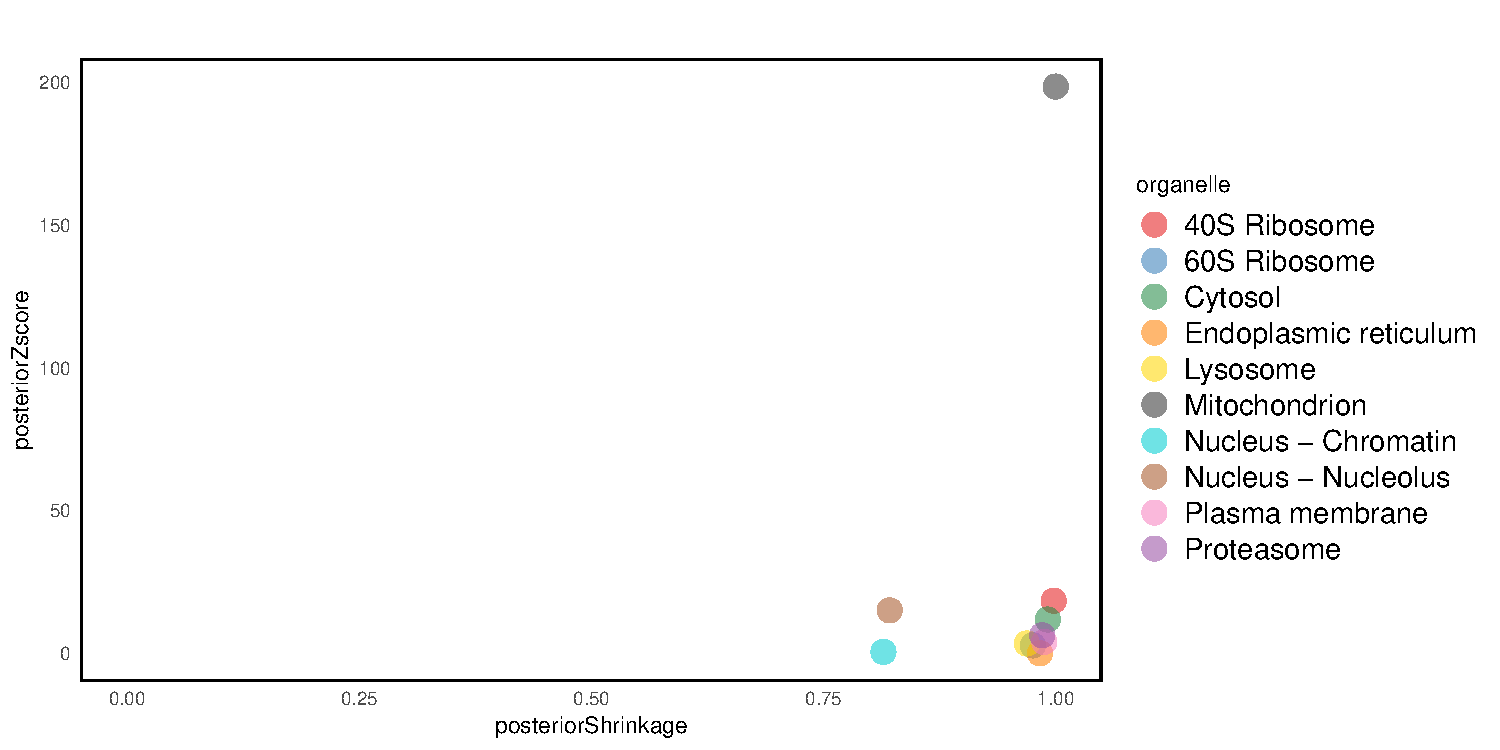
\includegraphics[width=0.7\linewidth]{F1000TAGMworkflow_rev1_files/figure-latex/unnamed-chunk-16-1} \caption{Scatter plot of the posterior shrinkage against the posterior z-score for the mixing proportions of the model}\label{fig:unnamed-chunk-16}
\end{figure}

We see that most parameter values concentrate in the lower right hand
corner of the plot, which suggests good shrinkage and calibration.
However, the parameter for the mitochondrion is located in the top right
of the plot suggesting the posterior deviates from the prior. The
biological interpretation for this is that the experiment resolved the
mitochondrial proteins extremely well and thus allocated many more
proteins to this class than perhaps we might have expected. This could
be remedied with a more informative prior. If we prefer to use an
informative prior, rather than a non-informative prior, it is practical
to use information from previous data. To demonstrate this, we consider
another experiment on mouse pluripotent stem cells and examine the
number of proteins that were allocated to each subcellular niche. The
code chunk below extracts this information from another spatial
proteomics experiment.

\begin{Shaded}
\begin{Highlighting}[]
\KeywordTok{data}\NormalTok{(}\StringTok{"hyperLOPIT2015"}\NormalTok{)}
\NormalTok{priordata <-}\StringTok{ }\KeywordTok{table}\NormalTok{(}\KeywordTok{fData}\NormalTok{(hyperLOPIT2015)}\OperatorTok{$}\NormalTok{final.assignment)}
\NormalTok{priordata}
\end{Highlighting}
\end{Shaded}

\begin{verbatim}
## 
##                          40S Ribosome                          60S Ribosome 
##                                    48                                    62 
##                    Actin cytoskeleton                               Cytosol 
##                                    46                                   339 
## Endoplasmic reticulum/Golgi apparatus                              Endosome 
##                                   426                                    60 
##                  Extracellular matrix                              Lysosome 
##                                    17                                    80 
##                         Mitochondrion                   Nucleus - Chromatin 
##                                   585                                   297 
##               Nucleus - Non-chromatin                            Peroxisome 
##                                   396                                    25 
##                       Plasma membrane                            Proteasome 
##                                   392                                    34 
##                               unknown 
##                                  2225
\end{verbatim}

It is clear that the allocations are not uniformly distributed across
the classes and that the mitochondrion has more allocations than the
other subcellular niches. However, we also do not have prior information
on all the classes. The Dirichlet distribution can be interpreted as
specifiying the prior relative proportions of the number of proteins
allocated to each niche. For the classes where we have no information,
we assume equal uniform allocations. First, we compute the number of
proteins in this experiment. Then create a vector with proteins
allocated equally to each class.

\begin{Shaded}
\begin{Highlighting}[]
\NormalTok{N <-}\StringTok{ }\KeywordTok{nrow}\NormalTok{(}\KeywordTok{unknownMSnSet}\NormalTok{(E14TG2aR)) }\CommentTok{# number of proteins}
\NormalTok{K <-}\StringTok{ }\KeywordTok{length}\NormalTok{(}\KeywordTok{getMarkerClasses}\NormalTok{(E14TG2aR)) }\CommentTok{# number of subcellular niches}
\NormalTok{beta_uninformed <-}\StringTok{ }\KeywordTok{rep}\NormalTok{(N}\OperatorTok{/}\NormalTok{K, K) }\CommentTok{# uninformative beta0, proteins allocated symmetrically}
\KeywordTok{names}\NormalTok{(beta_uninformed) <-}\StringTok{ }\KeywordTok{getMarkerClasses}\NormalTok{(E14TG2aR)}
\end{Highlighting}
\end{Shaded}

The code chunk below extracts the data for which we have prior
information.

\begin{Shaded}
\begin{Highlighting}[]
\NormalTok{shared_info <-}\StringTok{ }\KeywordTok{intersect}\NormalTok{(}\KeywordTok{getMarkerClasses}\NormalTok{(hyperLOPIT2015), }\KeywordTok{getMarkerClasses}\NormalTok{(E14TG2aR))}
\NormalTok{informativePrior <-}\StringTok{ }\NormalTok{priordata[shared_info] }\CommentTok{# extracts useful information from other dataset}
\end{Highlighting}
\end{Shaded}

We then reweight the prior number of proteins allocated to each class by
their relative proportions in the other dataset. We then use this
information to create an informative prior.

\begin{Shaded}
\begin{Highlighting}[]
\NormalTok{beta_informed <-}\StringTok{ }\NormalTok{beta_uninformed}
\NormalTok{beta_informed[shared_info] <-}\StringTok{ }\KeywordTok{sum}\NormalTok{(beta_uninformed[shared_info]) }\OperatorTok{*}\StringTok{ }\NormalTok{informativePrior}\OperatorTok{/}\KeywordTok{sum}\NormalTok{(informativePrior)}
\end{Highlighting}
\end{Shaded}

Now, we can check that this prior has captured our beliefs correctly,
mainly that the mitchondrion should have more allocations than the other
subcellular niches and that distribution is not symmetric. To do this,
we simulate \(10000\) values from the informative prior and compute the
expected (prior) number of proteins allocated to each niche.

\begin{Shaded}
\begin{Highlighting}[]
\NormalTok{prior_simulation <-}\StringTok{ }\KeywordTok{colMeans}\NormalTok{(gtools}\OperatorTok{::}\KeywordTok{rdirichlet}\NormalTok{(}\DataTypeTok{n =} \DecValTok{10000}\NormalTok{, }\DataTypeTok{alpha =}\NormalTok{ beta_informed) }\OperatorTok{*}\StringTok{ }\NormalTok{N)}
\KeywordTok{names}\NormalTok{(prior_simulation) <-}\StringTok{ }\KeywordTok{getMarkerClasses}\NormalTok{(E14TG2aR)}
\NormalTok{prior_simulation}
\end{Highlighting}
\end{Shaded}

\begin{verbatim}
##          40S Ribosome          60S Ribosome               Cytosol 
##              34.72586              44.99799             245.62171 
## Endoplasmic reticulum              Lysosome         Mitochondrion 
##             166.50286              57.99014             423.32247 
##   Nucleus - Chromatin   Nucleus - Nucleolus       Plasma membrane 
##             215.53612             166.26266             283.48035 
##            Proteasome 
##              24.55985
\end{verbatim}

\begin{Shaded}
\begin{Highlighting}[]
\KeywordTok{par}\NormalTok{(}\DataTypeTok{mar =} \KeywordTok{c}\NormalTok{(}\FloatTok{11.5}\NormalTok{, }\FloatTok{6.5}\NormalTok{, }\FloatTok{0.5}\NormalTok{, }\FloatTok{0.5}\NormalTok{), }\DataTypeTok{mgp =} \KeywordTok{c}\NormalTok{(}\DecValTok{10}\NormalTok{, }\DecValTok{1}\NormalTok{, }\DecValTok{0}\NormalTok{))}
\KeywordTok{barplot}\NormalTok{(prior_simulation, }\DataTypeTok{las =} \DecValTok{2}\NormalTok{, }\DataTypeTok{col =} \StringTok{"darkgreen"}\NormalTok{, }\DataTypeTok{xlab =} \StringTok{"sub-cellular niche"}\NormalTok{, }\DataTypeTok{ylab =} \StringTok{"prior expected number of allocations"}\NormalTok{)}
\end{Highlighting}
\end{Shaded}

\begin{figure}
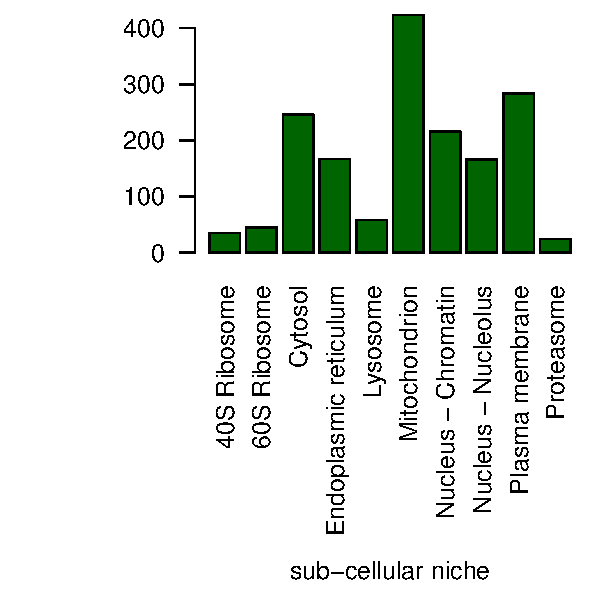
\includegraphics[width=1\linewidth]{F1000TAGMworkflow_rev1_files/figure-latex/priorpredict-1} \caption{A barplot showing the expected (prior) number of proteins allocated to each niche }\label{fig:priorpredict}
\end{figure}

It is clear that this prior captures the information that the
mitochondrion has more allocations than the other subcellular niches and
that the allocations across the classes are not symmetric. It is useful
to note that many spatial proteomics datasets can be found in the
\texttt{pRolocdata} package from which useful information could be
extracted.

\hypertarget{prior-on-the-proportion-of-outlier-proteins}{%
\subsubsection{Prior on the proportion of outlier
proteins}\label{prior-on-the-proportion-of-outlier-proteins}}

The prior for the proportion of outlier proteins is a
\(\mathcal{B}(u, v)\) distribution. The default for \(u = 2\) and the
default for \(v = 10\). This represents the reasonable belief that
\(\frac{u}{u + v} = \frac{1}{6}\) proteins \emph{a priori} might be an
outlier and we believe is unlikely that more than \(50\%\) of proteins
are outliers, which was elicited from expert domain knowledge and
analysis of previous datasets. Decreasing the value of \(v\), represents
more uncertainty about the number of proteins that are outliers.

To visualise that this prior captures these beliefs, we simulate from
the prior and produce a histogram.

\begin{Shaded}
\begin{Highlighting}[]
\NormalTok{x <-}\StringTok{ }\KeywordTok{rbeta}\NormalTok{(}\DataTypeTok{n =} \DecValTok{1500}\NormalTok{, }\DataTypeTok{shape1 =} \DecValTok{2}\NormalTok{, }\DataTypeTok{shape2 =} \DecValTok{10}\NormalTok{)}
\NormalTok{gg <-}\StringTok{ }\KeywordTok{ggplot}\NormalTok{(}\KeywordTok{data.frame}\NormalTok{(x), }\KeywordTok{aes}\NormalTok{(x)) }\OperatorTok{+}\StringTok{ }\KeywordTok{geom_histogram}\NormalTok{(}\DataTypeTok{fill =} \StringTok{"darkgreen"}\NormalTok{, }\DataTypeTok{col =} \StringTok{"black"}\NormalTok{) }\OperatorTok{+}\StringTok{ }
\StringTok{      }\KeywordTok{theme_minimal}\NormalTok{() }\OperatorTok{+}\StringTok{ }
\StringTok{      }\KeywordTok{theme}\NormalTok{(}\DataTypeTok{panel.grid.major =} \KeywordTok{element_blank}\NormalTok{(), }\DataTypeTok{panel.grid.minor =} \KeywordTok{element_blank}\NormalTok{(),}
           \DataTypeTok{panel.border =} \KeywordTok{element_rect}\NormalTok{(}\DataTypeTok{colour =} \StringTok{"black"}\NormalTok{, }\DataTypeTok{fill =} \OtherTok{NA}\NormalTok{, }\DataTypeTok{size =} \DecValTok{1}\NormalTok{),}
           \DataTypeTok{plot.title =} \KeywordTok{element_text}\NormalTok{(}\DataTypeTok{hjust =} \FloatTok{0.5}\NormalTok{, }\DataTypeTok{size =} \DecValTok{20}\NormalTok{),}
           \DataTypeTok{legend.text=}\KeywordTok{element_text}\NormalTok{(}\DataTypeTok{size =} \DecValTok{14}\NormalTok{)) }\OperatorTok{+}\StringTok{ }
\StringTok{      }\KeywordTok{ggtitle}\NormalTok{(}\DataTypeTok{label =} \StringTok{"Histogram of simulations from the prior"}\NormalTok{) }\OperatorTok{+}\StringTok{ }\KeywordTok{xlim}\NormalTok{(}\KeywordTok{c}\NormalTok{(}\OperatorTok{-}\FloatTok{0.05}\NormalTok{, }\DecValTok{1}\NormalTok{))}
\NormalTok{gg}
\end{Highlighting}
\end{Shaded}

\begin{verbatim}
## `stat_bin()` using `bins = 30`. Pick better value with `binwidth`.
\end{verbatim}

\begin{verbatim}
## Warning: Removed 2 rows containing missing values (geom_bar).
\end{verbatim}

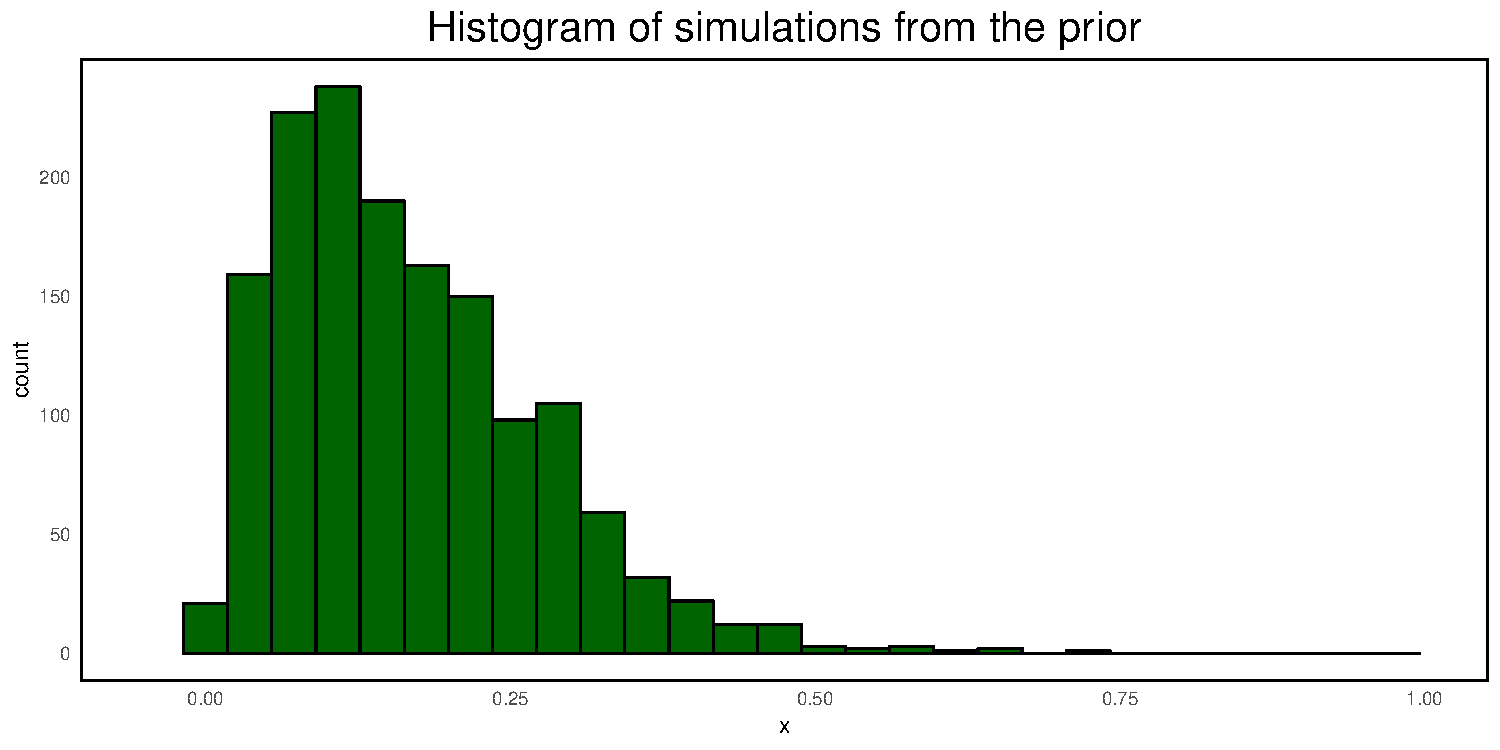
\includegraphics[width=0.7\linewidth]{F1000TAGMworkflow_rev1_files/figure-latex/unnamed-chunk-22-1}

The probability that more than \(50\%\) of the proteins are outliers is
small but non-zero. The probability there are fewer than \(1\%\)
outliers is also small. These quantiles can be used to calibrate the
prior beliefs.

\begin{Shaded}
\begin{Highlighting}[]
\KeywordTok{pbeta}\NormalTok{(}\FloatTok{0.5}\NormalTok{, }\DataTypeTok{shape1 =} \DecValTok{2}\NormalTok{, }\DataTypeTok{shape2 =} \DecValTok{10}\NormalTok{, }\DataTypeTok{lower.tail =} \OtherTok{FALSE}\NormalTok{) }\CommentTok{# more than 50% outliers}
\end{Highlighting}
\end{Shaded}

\begin{verbatim}
## [1] 0.005859375
\end{verbatim}

\begin{Shaded}
\begin{Highlighting}[]
\KeywordTok{pbeta}\NormalTok{(}\FloatTok{0.01}\NormalTok{, }\DataTypeTok{shape1 =} \DecValTok{2}\NormalTok{, }\DataTypeTok{shape2 =} \DecValTok{10}\NormalTok{, }\DataTypeTok{lower.tail =} \OtherTok{TRUE}\NormalTok{) }\CommentTok{# fewer than 1% outliers}
\end{Highlighting}
\end{Shaded}

\begin{verbatim}
## [1] 0.005179717
\end{verbatim}

Now we turn to the posterior distribution for this quantity of interest
and overlay onto the prior.

\begin{Shaded}
\begin{Highlighting}[]
\NormalTok{out <-}\StringTok{ }\KeywordTok{mcmc_get_outliers}\NormalTok{(e14Tagm_converged_pooled)}
\NormalTok{propout <-}\StringTok{ }\NormalTok{out[[}\DecValTok{1}\NormalTok{]]}\OperatorTok{/}\KeywordTok{nrow}\NormalTok{(}\KeywordTok{unknownMSnSet}\NormalTok{(E14TG2aR))}
\NormalTok{df <-}\StringTok{ }\KeywordTok{data.frame}\NormalTok{(}\DataTypeTok{x =} \KeywordTok{c}\NormalTok{(x, propout), }\DataTypeTok{y =} \KeywordTok{as.factor}\NormalTok{(}\KeywordTok{rep}\NormalTok{(}\KeywordTok{c}\NormalTok{(}\StringTok{"prior"}\NormalTok{, }\StringTok{"posterior"}\NormalTok{), }\DataTypeTok{each =} \DecValTok{1500}\NormalTok{)))}
\NormalTok{gg <-}\StringTok{ }\KeywordTok{ggplot}\NormalTok{(df, }\KeywordTok{aes}\NormalTok{(}\DataTypeTok{x =}\NormalTok{ x, }\DataTypeTok{fill =}\NormalTok{ y)) }\OperatorTok{+}\StringTok{ }\KeywordTok{geom_histogram}\NormalTok{(}\DataTypeTok{alpha =} \FloatTok{0.7}\NormalTok{, }\DataTypeTok{col =} \StringTok{"black"}\NormalTok{, }\DataTypeTok{position =} \StringTok{"identity"}\NormalTok{, }\DataTypeTok{bins =} \DecValTok{40}\NormalTok{) }\OperatorTok{+}\StringTok{ }
\StringTok{      }\KeywordTok{theme_minimal}\NormalTok{() }\OperatorTok{+}\StringTok{ }
\StringTok{      }\KeywordTok{theme}\NormalTok{(}\DataTypeTok{panel.grid.major =} \KeywordTok{element_blank}\NormalTok{(), }\DataTypeTok{panel.grid.minor =} \KeywordTok{element_blank}\NormalTok{(),}
           \DataTypeTok{panel.border =} \KeywordTok{element_rect}\NormalTok{(}\DataTypeTok{colour =} \StringTok{"black"}\NormalTok{, }\DataTypeTok{fill =} \OtherTok{NA}\NormalTok{, }\DataTypeTok{size =} \DecValTok{1}\NormalTok{),}
           \DataTypeTok{plot.title =} \KeywordTok{element_text}\NormalTok{(}\DataTypeTok{hjust =} \FloatTok{0.5}\NormalTok{, }\DataTypeTok{size =} \DecValTok{20}\NormalTok{),}
           \DataTypeTok{legend.text=}\KeywordTok{element_text}\NormalTok{(}\DataTypeTok{size =} \DecValTok{14}\NormalTok{)) }\OperatorTok{+}\StringTok{ }\KeywordTok{labs}\NormalTok{(}\DataTypeTok{fill =} \StringTok{"Distribution"}\NormalTok{) }\OperatorTok{+}\StringTok{ }
\StringTok{      }\KeywordTok{scale_fill_manual}\NormalTok{(}\DataTypeTok{values =} \KeywordTok{c}\NormalTok{(}\StringTok{"purple"}\NormalTok{, }\StringTok{"darkgreen"}\NormalTok{)) }\OperatorTok{+}\StringTok{ }
\StringTok{      }\KeywordTok{ggtitle}\NormalTok{(}\DataTypeTok{label =} \StringTok{"Histogram of samples from the prior and posterior"}\NormalTok{) }\OperatorTok{+}\StringTok{ }\KeywordTok{xlim}\NormalTok{(}\KeywordTok{c}\NormalTok{(}\OperatorTok{-}\FloatTok{0.05}\NormalTok{, }\DecValTok{1}\NormalTok{))}
\NormalTok{gg}
\end{Highlighting}
\end{Shaded}

\begin{verbatim}
## Warning: Removed 4 rows containing missing values (geom_bar).
\end{verbatim}

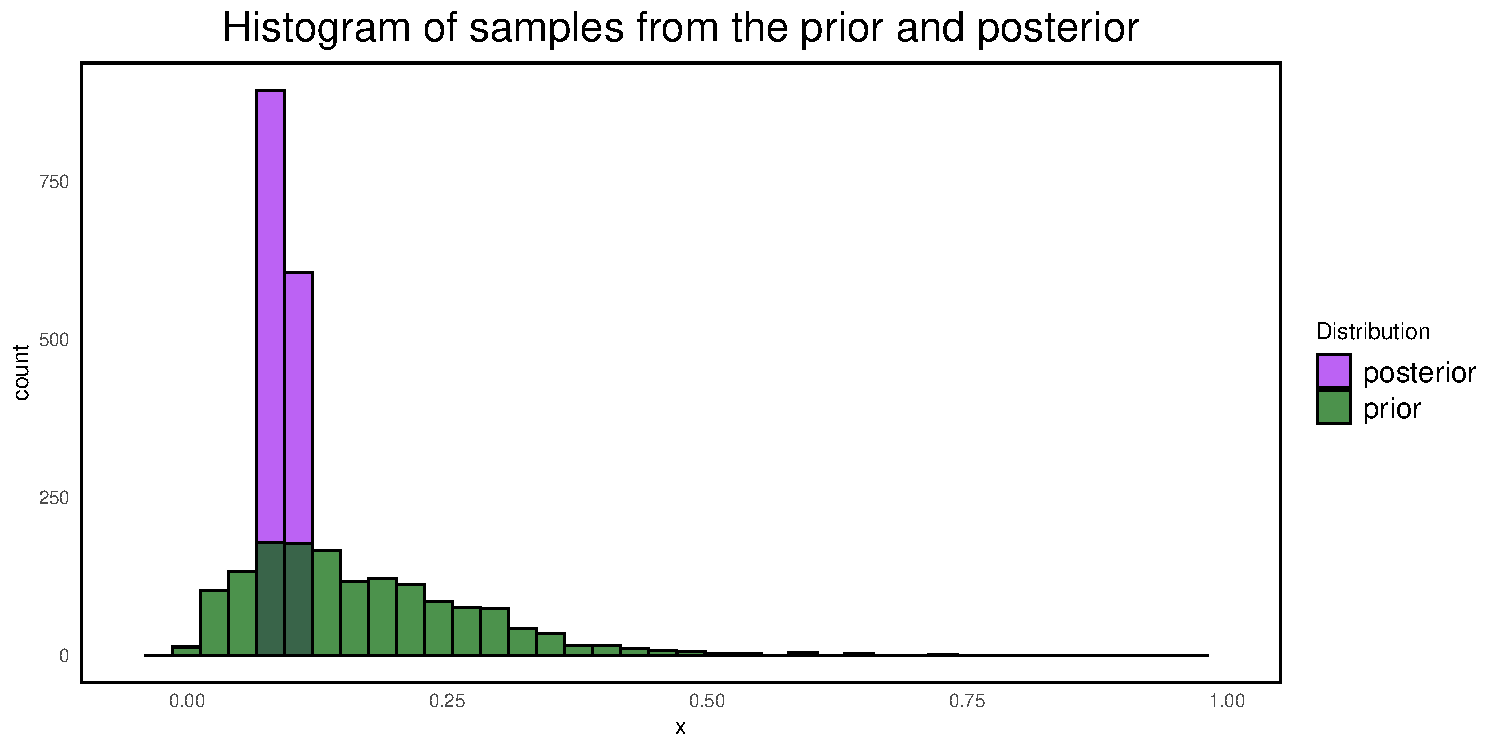
\includegraphics[width=0.7\linewidth]{F1000TAGMworkflow_rev1_files/figure-latex/unnamed-chunk-24-1}

It is clear that the prior and posterior concentrate in the same region,
and are thus not in conflict. The variance of the posterior is clearly
smaller than that of the prior and so there is high posterior shrinkage.
One could argue that the prior is too diffuse to provide regularisation;
however, specifying a tighter prior risks biasing the model away from
the data generating mechanism.

\hypertarget{analysis-visualisation-and-interpretation-of-results}{%
\subsection{Analysis, visualisation and interpretation of
results}\label{analysis-visualisation-and-interpretation-of-results}}

Now that we have a single pooled chain of samples from a converged MCMC
algorithm, we can begin to analyse the results. Preliminary analysis
includes visualising the allocated organelle and localisation
probability of each protein to its most probable organelle, as shown on
figure @ref(fig:mcmcpca).

\begin{Shaded}
\begin{Highlighting}[]
\KeywordTok{layout}\NormalTok{(}\KeywordTok{matrix}\NormalTok{(}\KeywordTok{c}\NormalTok{(}\DecValTok{1}\NormalTok{,}\DecValTok{1}\NormalTok{,}\DecValTok{2}\NormalTok{,}\DecValTok{2}\NormalTok{), }\DataTypeTok{nrow =} \DecValTok{4}\NormalTok{, }\DataTypeTok{ncol =} \DecValTok{1}\NormalTok{, }\DataTypeTok{byrow =} \OtherTok{TRUE}\NormalTok{))}
\KeywordTok{plot2D}\NormalTok{(E14TG2aR, }\DataTypeTok{fcol =} \StringTok{"tagm.mcmc.allocation"}\NormalTok{,}
       \DataTypeTok{cex =} \KeywordTok{fData}\NormalTok{(E14TG2aR)}\OperatorTok{$}\NormalTok{tagm.mcmc.probability,}
       \DataTypeTok{main =} \StringTok{"TAGM MCMC allocations"}\NormalTok{)}
\KeywordTok{addLegend}\NormalTok{(E14TG2aR, }\DataTypeTok{fcol =} \StringTok{"markers"}\NormalTok{,}
          \DataTypeTok{where =} \StringTok{"topleft"}\NormalTok{, }\DataTypeTok{ncol =} \DecValTok{2}\NormalTok{, }\DataTypeTok{cex =} \FloatTok{0.6}\NormalTok{)}

\KeywordTok{plot2D}\NormalTok{(E14TG2aR, }\DataTypeTok{fcol =} \StringTok{"tagm.mcmc.allocation"}\NormalTok{,}
       \DataTypeTok{cex =} \KeywordTok{fData}\NormalTok{(E14TG2aR)}\OperatorTok{$}\NormalTok{tagm.mcmc.mean.shannon,}
       \DataTypeTok{main =} \StringTok{"Visualising global uncertainty"}\NormalTok{)}
\KeywordTok{addLegend}\NormalTok{(E14TG2aR, }\DataTypeTok{fcol =} \StringTok{"markers"}\NormalTok{,}
          \DataTypeTok{where =} \StringTok{"topleft"}\NormalTok{, }\DataTypeTok{ncol =} \DecValTok{2}\NormalTok{, }\DataTypeTok{cex =} \FloatTok{0.6}\NormalTok{)}
\end{Highlighting}
\end{Shaded}

\begin{figure}
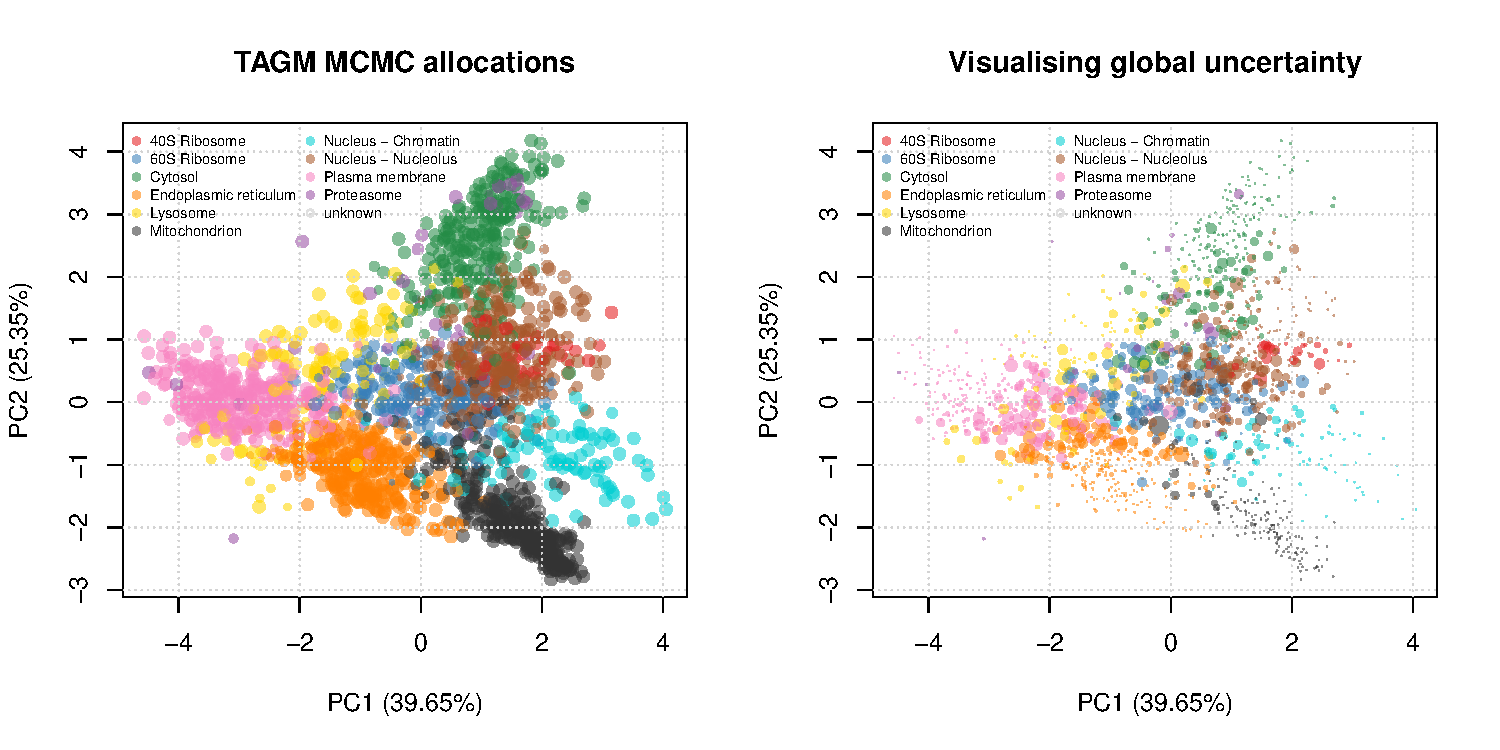
\includegraphics[width=1\linewidth]{F1000TAGMworkflow_rev1_files/figure-latex/mcmcpca-1} \caption{TAGM MCMC allocations. In the upper plot, pointer sizes have been scaled based on allocation probabilities. On the lower plot, the pointer sizes have been scaled based on the global uncertainty using the mean Shannon entropy.}\label{fig:mcmcpca}
\end{figure}

We can visualise other summaries of the data including a Monte-Carlo
averaged Shannon entropy, as shown in figure @ref(fig:mcmcpca) on the
right. This is a measure of uncertainty and proteins with greater
Shannon entropy have more uncertainty in their localisation. The Shannon
Entropy (and hence uncertainty) is greatest when all localisation are
equiprobable and lowest when the probabilities are concentrated on a
single localisation. For additional discussion, we refer readers to
Crook et al. (2018) and Oliver M Crook et al. (2019) and references
therein. We observe global patterns of uncertainty, particularly in
areas where organelle boundaries overlap. There are also regions of low
uncertainty indicating little doubt about the localisation of these
proteins.

We are also interested in the relationship between localisation
probability to the most probable class and the Shannon entropy. Even
though the two quantities are evidently correlated there is still
considerable spread. Thus it is important to base inference not only on
localisation probability but also a measure of uncertainty, for example
the Shannon entropy. Proteins with low Shannon entropy have low
uncertainty in their localisation, whilst those with higher Shannon
entropy have uncertain localisation. Since multi-localised proteins have
uncertain localisation to a single subcellular niche, exploring the
Shannon can aid in identifying multi-localised proteins. Examples of
well characterised multi-localising proteins from the literature are
discussed in (Crook et al. 2018). The interpretation of uncertain
allocations in relation to multi-localisation is further discussed in
(Crook et al. 2018; Oliver M Crook et al. 2019).

\begin{Shaded}
\begin{Highlighting}[]
\NormalTok{cls <-}\StringTok{ }\KeywordTok{getStockcol}\NormalTok{()[}\KeywordTok{as.factor}\NormalTok{(}\KeywordTok{fData}\NormalTok{(E14TG2aR)}\OperatorTok{$}\NormalTok{tagm.mcmc.allocation)]}
\KeywordTok{plot}\NormalTok{(}\KeywordTok{fData}\NormalTok{(E14TG2aR)}\OperatorTok{$}\NormalTok{tagm.mcmc.probability,}
     \KeywordTok{fData}\NormalTok{(E14TG2aR)}\OperatorTok{$}\NormalTok{tagm.mcmc.mean.shannon,}
     \DataTypeTok{col =}\NormalTok{ cls, }\DataTypeTok{pch =} \DecValTok{19}\NormalTok{,}
     \DataTypeTok{xlab =} \StringTok{"Localisation probability"}\NormalTok{,}
     \DataTypeTok{ylab =} \StringTok{"Shannon entropy"}\NormalTok{)}
\KeywordTok{addLegend}\NormalTok{(E14TG2aR, }\DataTypeTok{fcol =} \StringTok{"markers"}\NormalTok{,}
          \DataTypeTok{where =} \StringTok{"topright"}\NormalTok{, }\DataTypeTok{ncol =} \DecValTok{2}\NormalTok{, }\DataTypeTok{cex =} \FloatTok{0.6}\NormalTok{)}
\end{Highlighting}
\end{Shaded}

\begin{figure}
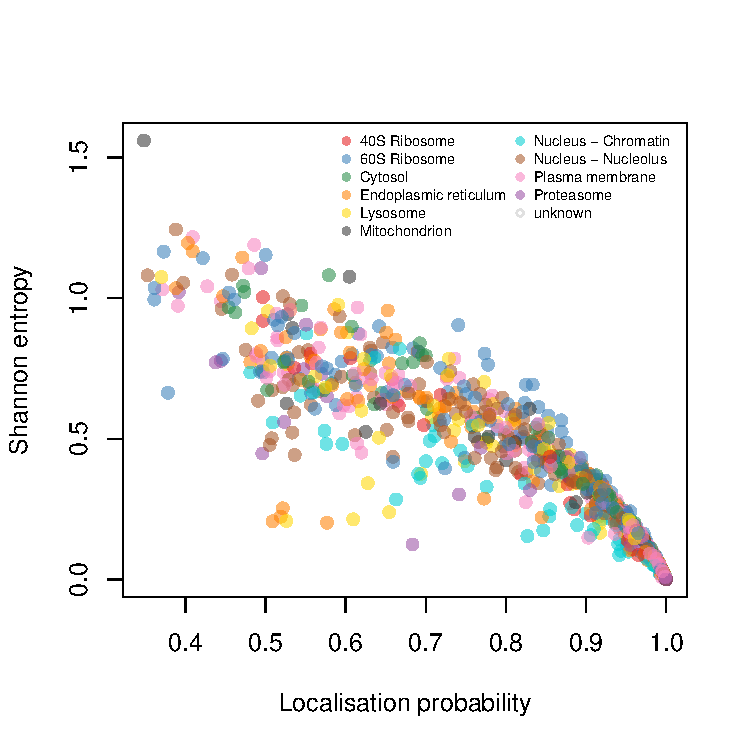
\includegraphics[width=0.7\linewidth]{F1000TAGMworkflow_rev1_files/figure-latex/probvsentr-1} \caption{Shannon entropy and localisation probability.}\label{fig:probvsentr}
\end{figure}

There are further ways in which we can visualise the uncertainty
quantified by the Bayesian analysis. For example, we can use the samples
from the MCMC algorithm to visualise the uncertainty in the mean
localisation of each organelle/niche on a PCA plot. At each iteration of
the MCMC, we compute the mean for each organelle as the mean of all
associated proteins to that organelle. These data are then projected on
to the PCA plot, having aligned them across the random samples (see
(Borg and Groenen 2003), as well as (Ren et al. 2017) and (Nguyen and
Holmes 2019) for similar examples).

\begin{Shaded}
\begin{Highlighting}[]
\KeywordTok{nicheMeans2D}\NormalTok{(}\DataTypeTok{object =}\NormalTok{ E14TG2aR, }\DataTypeTok{params =}\NormalTok{ e14Tagm_converged_pooled[[}\DecValTok{1}\NormalTok{]], }\DataTypeTok{prior =}\NormalTok{ e14Tagm_converged_pooled}\OperatorTok{@}\NormalTok{priors)}
\end{Highlighting}
\end{Shaded}

\begin{figure}
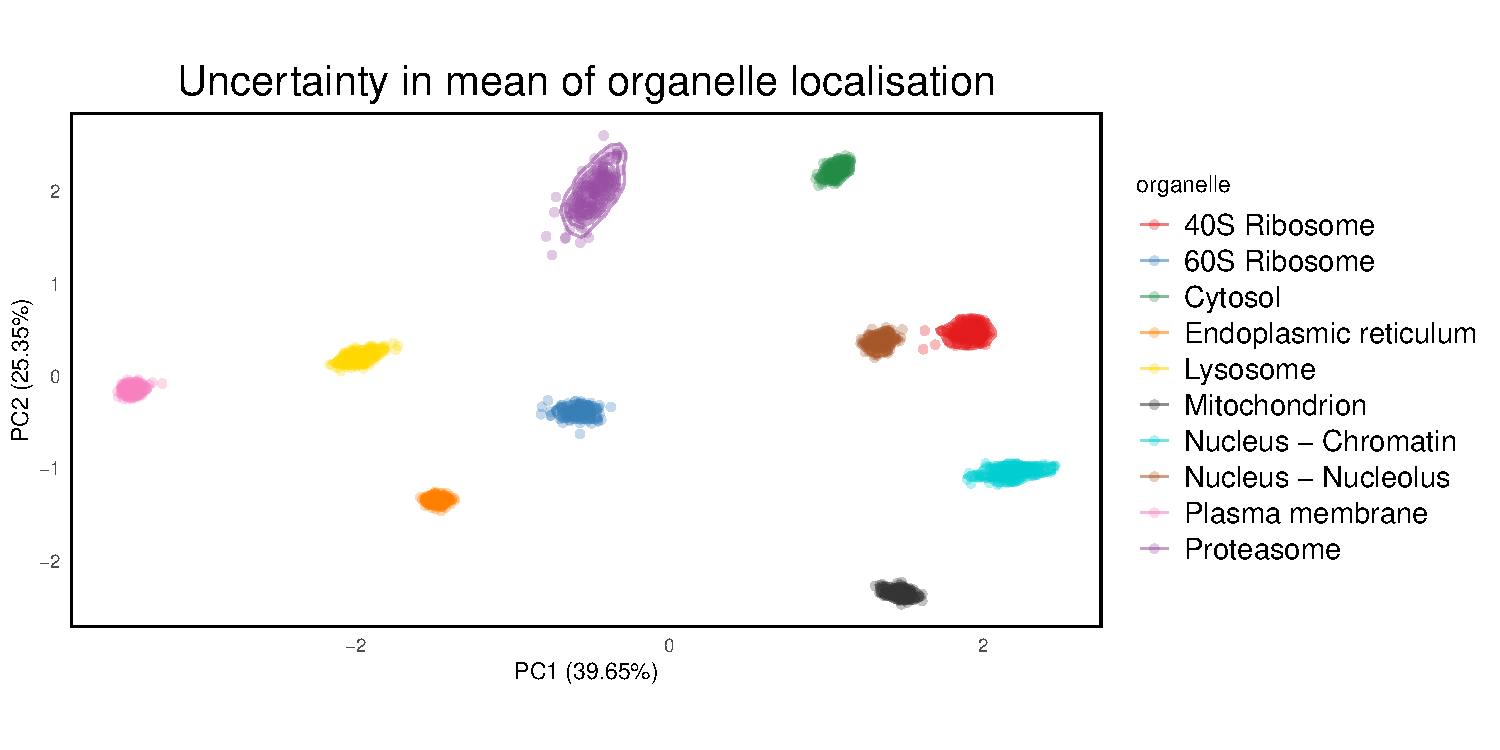
\includegraphics[width=0.7\linewidth]{F1000TAGMworkflow_rev1_files/figure-latex/nicheuncertainty-1} \caption{Visualising uncertainty in the mean of each subcellular niche. The pointers correspond to results from different iterations of the MCMC algorithm and are coloured according to the corresponding subcellular niche}\label{fig:nicheuncertainty}
\end{figure}

The main quantity of interest is posterior localisation probability of
each protein to each organelle. However, visualising how these
probabilities vary in different regions of data space are be
challenging, especially with large numbers of proteins. Furthermore,
interrogating individual proteins one by one can be cumbersome. Thus, we
consider visualising how the probabilities vary across different regions
of the PCA plot. To perform this analysis, we first compute the
underlying coordinates of the whole data in PC space. We proceed by
linearly interpolating a regular grid in this coordinate system. To
obtain the localisation probabilties on this grid, we use a
Nadaraya-Watson kernel smoother (Nadaraya 1964; Watson 1964) with
Wendland covariance (Wendland 1995), where a fast Fourier transform is
used to accelerate computations (Stein 1999; Gneiting 2002). A contour
plot, in the PC coordinates, of these probabilities is then visualised,
where the distribution for each organelle is coloured accordingly. The
code chunk below produces this plot.

\begin{Shaded}
\begin{Highlighting}[]
\KeywordTok{spatial2D}\NormalTok{(}\DataTypeTok{object =}\NormalTok{ E14TG2aR)}
\end{Highlighting}
\end{Shaded}

\begin{figure}
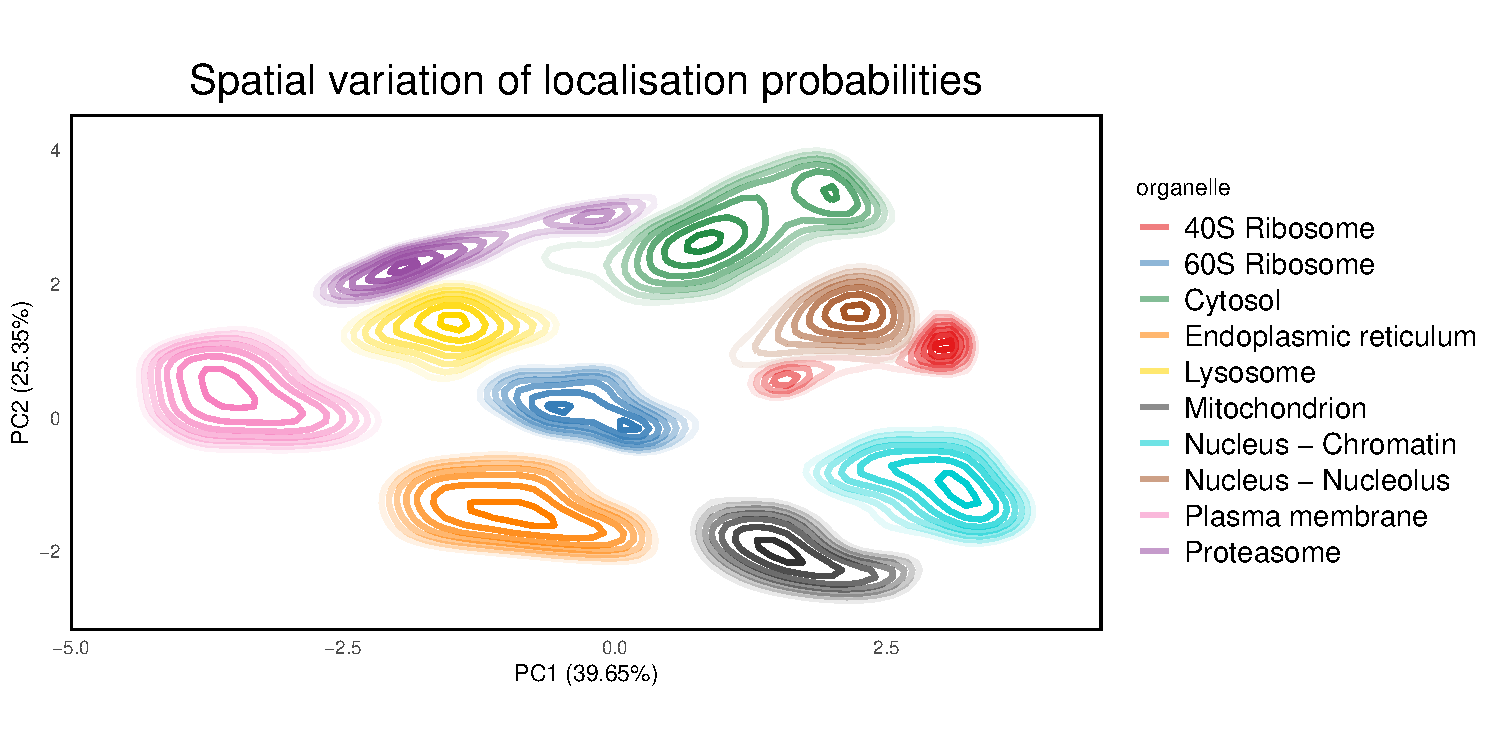
\includegraphics[width=0.7\linewidth]{F1000TAGMworkflow_rev1_files/figure-latex/spatialplot-1} \caption{Visualising how the posterior localisation  probabilities vary smoothly across different regions of the PCA plot. The colours correspond the different subcellular niches. The inner most contour corresponds to a probability of 0.99 and the following contour to 0.95, with each subsequent contour descreasing in 0.05 increments}\label{fig:spatialplot}
\end{figure}

Aside from global visualisation of the data, we can also interrogate
each individual protein. As illustrated on figure @ref(fig:probdists1),
we can obtain the full posterior distribution of localisation
probabilities for each protein from the
\texttt{e14Tagm\_converged\_pooled} object. We can use the \texttt{plot}
generic on the \texttt{MCMCParams} object to obtain a violin plot of the
localisation distribution. Simply providing the name of the protein in
the second argument produces the plot for that protein. The solute
carrier transporter protein E9QMX3, also referred to as Slc15a1, is most
probably localised to plasma membrane in line with its role as a
transmembrane transporter but also shows some uncertainty, potentially
also localising to other comparments. The first violin plot visualises
this uncertainty. The protein Q3V1Z5 is a supposed constitute of the 40S
ribosome and has poor UniProt annotation with evidence only at the
transcript level. From the plot below it is clear that Q3V1Z5 is a
ribosomal associated protein, but it previous localisation has only been
computational inferred and here we provide experimental evidence of a
ribosomal annotation. Thus, quantifying uncertainty recovers important
additional annotations.

\begin{Shaded}
\begin{Highlighting}[]
\KeywordTok{plot}\NormalTok{(e14Tagm_converged_pooled, }\StringTok{"E9QMX3"}\NormalTok{)}
\KeywordTok{plot}\NormalTok{(e14Tagm_converged_pooled, }\StringTok{"Q3V1Z5"}\NormalTok{)}
\end{Highlighting}
\end{Shaded}

\begin{figure}
\centering
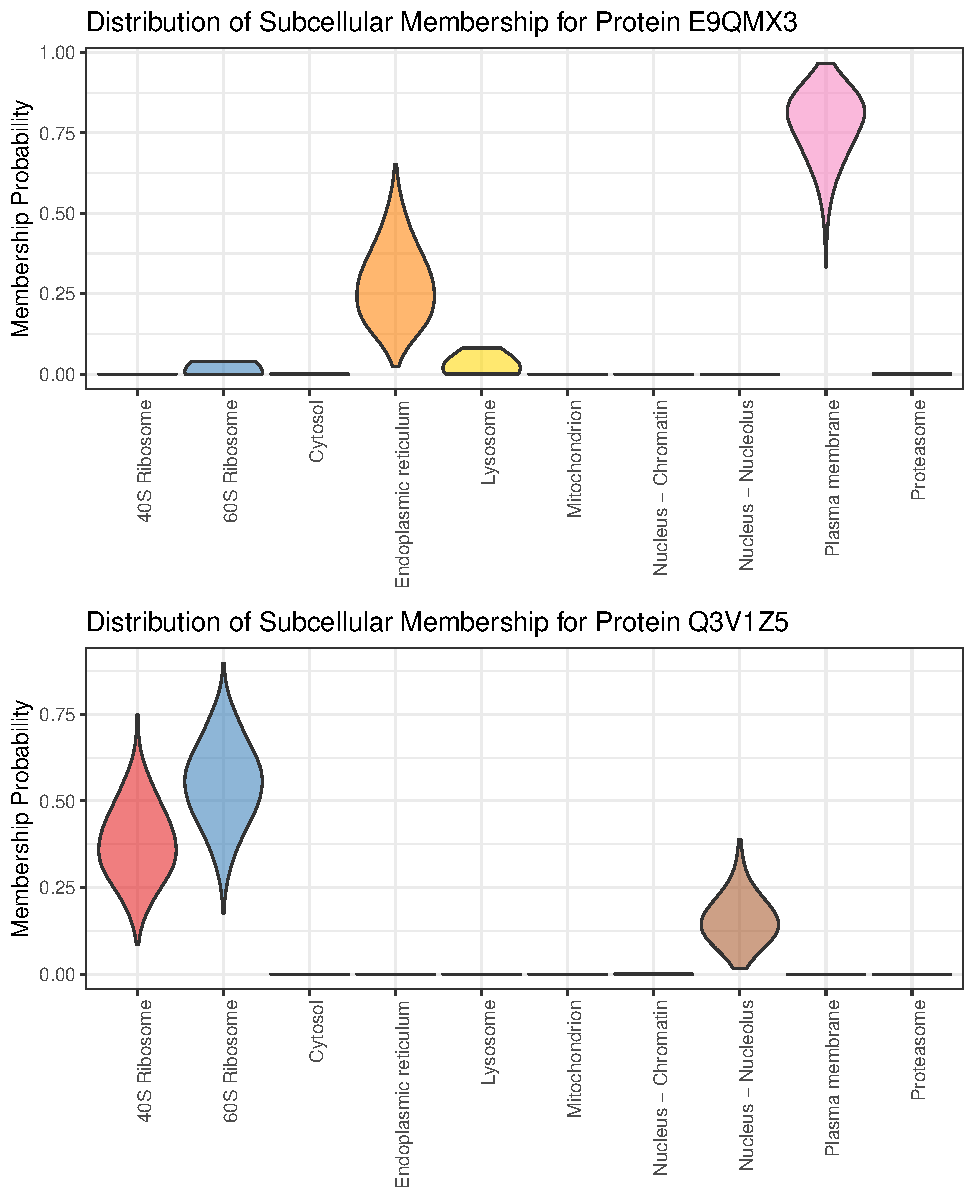
\includegraphics{F1000TAGMworkflow_rev1_files/figure-latex/probdists1-1.pdf}
\caption{Full posterior distribution of localisation probabilities for
individual proteins.}
\end{figure}

\hypertarget{discussion}{%
\section{Discussion}\label{discussion}}

The Bayesian analysis of biological data is of clear interest to many
because of its ability to provide richer information about the
experimental results. A fully Bayesian analysis differs from other
machine learning approaches, since it can quantify the uncertainty in
our inferences. Furthermore, we use a generative model to explicitly
describe the data, which makes inferences more interpretable compared to
the less interpretable outputs of black-box classifiers such as, for
example, support vector machines (SVM).

Bayesian analysis is often characterised by its provision of a
(posterior) probability distribution over the biological parameters of
interest, as opposed to single point estimate of these parameters. In
the case that is presented in this workflow, a Bayesian analysis
``computes'' a posterior probability distribution over the protein
localisation probabilities. These probability distributions can then be
rigorously interrogated for greater biological insight; in addition, it
may allow us to ask additional questions about the data, such as whether
a protein might be multi-localised.

Despite the wealth of information a Bayesian analysis can provide, the
uptake amongst cell biologists is still low. This is because a Bayesian
analysis presents a new set of challenges and little practical guidance
exists regarding how to address these challenges. Bayesian analyses
often rely on computatinally intensive approaches such as Markov-chain
Monte-Carlo (MCMC) and a practical understanding of these algorithms and
the interpretation of their output is a key barrier to their use. A
Bayesian analysis usually consists of three broad steps: (1) Data
pre-processing and algorithmic implementation, (2) assessing algorithmic
convergence and (3) summarising and visualising the results. This
workflow provides a set of tools to simplify these steps and provides
step-by-step guidance in the context of the analysis of spatial
proteomics data.

We have provided a workflow for the Bayesian analysis of spatial
proteomics using the \texttt{pRoloc} and \texttt{MSnbase} software. We
have demonstrated, in a step-by-step fashion, the challenges and
advantages associated with taking a Bayesian approach to data analysis.
We hope this workflow will help spatial proteomics practitioners to
apply our methods and will motivate others to create detailed
documentation for the Bayesian analysis of biological data.

\hypertarget{session-information}{%
\section{Session information}\label{session-information}}

Below, we provide a summary of all packages and versions used to
generate this document.

\begin{Shaded}
\begin{Highlighting}[]
\KeywordTok{sessionInfo}\NormalTok{()}
\end{Highlighting}
\end{Shaded}

\begin{verbatim}
## R version 4.0.0 (2020-04-24)
## Platform: x86_64-w64-mingw32/x64 (64-bit)
## Running under: Windows 10 x64 (build 18362)
## 
## Matrix products: default
## 
## Random number generation:
##  RNG:     Mersenne-Twister 
##  Normal:  Inversion 
##  Sample:  Rounding 
##  
## locale:
## [1] LC_COLLATE=English_United Kingdom.1252 
## [2] LC_CTYPE=English_United Kingdom.1252   
## [3] LC_MONETARY=English_United Kingdom.1252
## [4] LC_NUMERIC=C                           
## [5] LC_TIME=English_United Kingdom.1252    
## 
## attached base packages:
##  [1] grid      stats4    parallel  stats     graphics  grDevices utils    
##  [8] datasets  methods   base     
## 
## other attached packages:
##  [1] patchwork_1.0.0      pRolocdata_1.26.0    pRoloc_1.28.0       
##  [4] coda_0.19-3          fields_10.3          maps_3.3.0          
##  [7] spam_2.5-1           dotCall64_1.0-0      akima_0.6-2         
## [10] dplyr_1.0.0          ggplot2_3.3.0        mixtools_1.2.0      
## [13] BiocParallel_1.22.0  MLInterfaces_1.68.0  cluster_2.1.0       
## [16] annotate_1.66.0      XML_3.99-0.3         AnnotationDbi_1.50.0
## [19] IRanges_2.22.2       MSnbase_2.14.1       ProtGenerics_1.20.0 
## [22] S4Vectors_0.26.1     mzR_2.22.0           Rcpp_1.0.4.6        
## [25] Biobase_2.48.0       BiocGenerics_0.34.0 
## 
## loaded via a namespace (and not attached):
##   [1] colorspace_1.4-1      ellipsis_0.3.1        class_7.3-17         
##   [4] mclust_5.4.6          proxy_0.4-24          farver_2.0.3         
##   [7] hexbin_1.28.1         affyio_1.58.0         bit64_0.9-7          
##  [10] lubridate_1.7.8       prodlim_2019.11.13    mvtnorm_1.1-0        
##  [13] codetools_0.2-16      splines_4.0.0         ncdf4_1.17           
##  [16] doParallel_1.0.15     impute_1.62.0         knitr_1.28           
##  [19] LaplacesDemon_16.1.4  pROC_1.16.2           caret_6.0-86         
##  [22] kernlab_0.9-29        vsn_3.56.0            dbplyr_1.4.3         
##  [25] BiocManager_1.30.10   compiler_4.0.0        httr_1.4.1           
##  [28] sampling_2.8          assertthat_0.2.1      Matrix_1.2-18        
##  [31] limma_3.44.1          htmltools_0.4.0       prettyunits_1.1.1    
##  [34] tools_4.0.0           gtable_0.3.0          glue_1.4.1           
##  [37] affy_1.66.0           reshape2_1.4.4        rappdirs_0.3.1       
##  [40] MALDIquant_1.19.3     vctrs_0.3.0           preprocessCore_1.50.0
##  [43] nlme_3.1-147          iterators_1.0.12      timeDate_3043.102    
##  [46] gower_0.2.1           xfun_0.13             stringr_1.4.0        
##  [49] lpSolve_5.6.15        lifecycle_0.2.0       gtools_3.8.2         
##  [52] dendextend_1.13.4     zlibbioc_1.34.0       MASS_7.3-51.6        
##  [55] scales_1.1.1          ipred_0.9-9           pcaMethods_1.80.0    
##  [58] hms_0.5.3             RColorBrewer_1.1-2    yaml_2.2.1           
##  [61] curl_4.3              memoise_1.1.0         gridExtra_2.3        
##  [64] rpart_4.1-15          biomaRt_2.44.0        segmented_1.1-0      
##  [67] stringi_1.4.6         RSQLite_2.2.0         highr_0.8            
##  [70] randomForest_4.6-14   foreach_1.5.0         e1071_1.7-3          
##  [73] lava_1.6.7            rlang_0.4.6           pkgconfig_2.0.3      
##  [76] bitops_1.0-6          mzID_1.26.0           evaluate_0.14        
##  [79] lattice_0.20-41       purrr_0.3.4           labeling_0.3         
##  [82] recipes_0.1.12        bit_1.1-15.2          tidyselect_1.1.0     
##  [85] plyr_1.8.6            magrittr_1.5          R6_2.4.1             
##  [88] snow_0.4-3            generics_0.0.2        DBI_1.1.0            
##  [91] pillar_1.4.4          withr_2.2.0           nnet_7.3-14          
##  [94] survival_3.1-12       RCurl_1.98-1.2        sp_1.4-1             
##  [97] tibble_3.0.1          crayon_1.3.4          BiocFileCache_1.12.0 
## [100] rmarkdown_2.1         viridis_0.5.1         progress_1.2.2       
## [103] isoband_0.2.1         data.table_1.12.8     blob_1.2.1           
## [106] FNN_1.1.3             ModelMetrics_1.2.2.2  digest_0.6.25        
## [109] xtable_1.8-4          openssl_1.4.1         munsell_0.5.0        
## [112] viridisLite_0.3.0     askpass_1.1
\end{verbatim}

The source of this document, including the code necessary to reproduce
the analyses and figures is available in a public manuscript repository
on GitHub (O. Crook and Gatto 2019).

\hypertarget{data-availability}{%
\section{Data availability}\label{data-availability}}

The data used in this workflow was first published in Breckels \emph{et
al.} (2016) (Breckels, Holden, et al. 2016) and is available in the
\href{https://bioconductor.org/packages/release/data/experiment/html/pRolocdata.html}{pRolocdata}
package.

\hypertarget{software-availability}{%
\section{Software availability}\label{software-availability}}

Computational workflow for this study available from:
\url{https://github.com/ococrook/TAGMworkflow}

Archived source code at time of publication:
\url{https://doi.org/10.5281/zenodo.2593712} (Oliver M. Crook et al.
2019)

License: \href{https://creativecommons.org/licenses/by/4.0/legalcode}{CC
BY 4.0}

\hypertarget{grant-information}{%
\section{Grant information}\label{grant-information}}

PDWK was supported by the MRC (project reference MC\_UU\_00002/10 and
MC\_UU\_00002/13). LMB
\textless\textless\textless\textless\textless\textless\textless{} HEAD
was supported by a BBSRC Tools and Resources Development grant (Award
BB/N023129/1) and a Wellcome Trust Technology Development Grant (Grant
number 108441/Z/15/Z). OMC is a Wellcome Trust Mathematical Genomics and
Medicine student supported financially by the School of Clinical
Medicine, University of Cambridge. The funders had no role in study
design, data collection and analysis, decision to publish, or
preparation of the manuscript. ======= was supported by a BBSRC Tools
and Resources Development grant (Award BB/N023129/1) and a Wellcome
Trust Technology Development Grant (Grant number 108441/Z/15/Z). OMC is
a Wellcome Trust Mathematical Genomics and Medicine student supported
financially by the School of Clinical Medicine, University of Cambridge.

\emph{The funders had no role in study design, data collection and
analysis, decision to publish, or preparation of the manuscript.}
\textgreater\textgreater\textgreater\textgreater\textgreater\textgreater\textgreater{}
a294ccfa46042d30222c9a4b9655b4b00609cc48

\hypertarget{references}{%
\section*{References}\label{references}}
\addcontentsline{toc}{section}{References}

\hypertarget{refs}{}
\leavevmode\hypertarget{ref-Beltran:2016}{}%
Beltran, Pierre M Jean, Rommel A Mathias, and Ileana M Cristea. 2016.
``A Portrait of the Human Organelle Proteome in Space and Time During
Cytomegalovirus Infection.'' \emph{Cell Systems} 3 (4): 361--73.

\leavevmode\hypertarget{ref-Betancourt:2018}{}%
Betancourt, Michael. 2018. ``Calibrating Model-Based Inferences and
Decisions.'' \emph{arXiv Preprint arXiv:1803.08393}.

\leavevmode\hypertarget{ref-Borg:2003}{}%
Borg, Ingwer, and Patrick Groenen. 2003. ``Modern Multidimensional
Scaling: Theory and Applications.'' \emph{Journal of Educational
Measurement} 40 (3): 277--80.

\leavevmode\hypertarget{ref-Breckels:2013}{}%
Breckels, Lisa M, Laurent Gatto, Andy Christoforou, Arnoud J Groen,
Kathryn S Lilley, and Matthew WB Trotter. 2013. ``The Effect of
Organelle Discovery Upon Sub-Cellular Protein Localisation.''
\emph{Journal of Proteomics} 88: 129--40.

\leavevmode\hypertarget{ref-Breckels:2016}{}%
Breckels, Lisa M, Sean B Holden, David Wojnar, Claire M Mulvey, Andy
Christoforou, Arnoud Groen, Matthew WB Trotter, Oliver Kohlbacher,
Kathryn S Lilley, and Laurent Gatto. 2016. ``Learning from Heterogeneous
Data Sources: An Application in Spatial Proteomics.'' \emph{PLoS
Computational Biology} 12 (5): e1004920.

\leavevmode\hypertarget{ref-Breckels:2016b}{}%
Breckels, Lisa M, Claire M Mulvey, Kathryn S Lilley, and Laurent Gatto.
2016. ``A Bioconductor Workflow for Processing and Analysing Spatial
Proteomics Data.'' \emph{F1000Research} 5.

\leavevmode\hypertarget{ref-Brooks:1998}{}%
Brooks, Stephen P, and Andrew Gelman. 1998. ``General Methods for
Monitoring Convergence of Iterative Simulations.'' \emph{Journal of
Computational and Graphical Statistics} 7 (4): 434--55.

\leavevmode\hypertarget{ref-hyper}{}%
Christoforou, Andy, Claire M Mulvey, Lisa M Breckels, Aikaterini
Geladaki, Tracey Hurrell, Penelope C Hayward, Thomas Naake, et al. 2016.
``A Draft Map of the Mouse Pluripotent Stem Cell Spatial Proteome.''
\emph{Nature Communications} 7: 9992.

\leavevmode\hypertarget{ref-Cody:2013}{}%
Cody, Neal AL, Carole Iampietro, and Eric Lécuyer. 2013. ``The Many
Functions of mRNA Localization During Normal Development and Disease:
From Pillar to Post.'' \emph{Wiley Interdisciplinary Reviews:
Developmental Biology} 2 (6): 781--96.

\leavevmode\hypertarget{ref-oliver_m_crook_2019_2593712}{}%
Crook, Oliver M., Laurent Gatto, Paul DW Kirk, and Lisa Breckels. 2019.
``Ococrook/Tagmworkflow: F1000 Submission.''
\url{https://doi.org/10.5281/zenodo.2593712}.

\leavevmode\hypertarget{ref-Crook:2019}{}%
Crook, Oliver M, Kathryn S Lilley, Laurent Gatto, and Paul DW Kirk.
2019. ``Semi-Supervised Non-Parametric Bayesian Modelling of Spatial
Proteomics.'' \emph{arXiv Preprint arXiv:1903.02909}.

\leavevmode\hypertarget{ref-Crook:2018}{}%
Crook, Oliver M, Claire M Mulvey, Paul D W Kirk, Kathryn S Lilley, and
Laurent Gatto. 2018. ``A Bayesian Mixture Modelling Approach for Spatial
Proteomics.'' \emph{PLoS Comput. Biol.} 14 (11): e1006516.

\leavevmode\hypertarget{ref-ghrepo}{}%
Crook, OM, and L Gatto. 2019. ``A Bioconductor Workflow for the Bayesian
Analysis of Spatial Proteomics.'' \emph{GitHub Repository}.
\url{https://github.com/ococrook/TAGMworkflow}; GitHub.

\leavevmode\hypertarget{ref-Davies:2018}{}%
Davies, Alexandra K, Daniel N Itzhak, James R Edgar, Tara L Archuleta,
Jennifer Hirst, Lauren P Jackson, Margaret S Robinson, and Georg HH
Borner. 2018. ``AP-4 Vesicles Contribute to Spatial Control of Autophagy
via Rusc-Dependent Peripheral Delivery of Atg9a.'' \emph{Nature
Communications} 9: 3958.

\leavevmode\hypertarget{ref-De:2011}{}%
De Matteis, Maria Antonietta, and Alberto Luini. 2011. ``Mendelian
Disorders of Membrane Trafficking.'' \emph{New England Journal of
Medicine} 365 (10): 927--38.

\leavevmode\hypertarget{ref-EM:1977}{}%
Dempster, Arthur P, Nan M Laird, and Donald B Rubin. 1977. ``Maximum
Likelihood from Incomplete Data via the Em Algorithm.'' \emph{Journal of
the Royal Statistical Society. Series B (Methodological)}, 1--38.

\leavevmode\hypertarget{ref-Dunkley:2006}{}%
Dunkley, Tom PJ, Svenja Hester, Ian P Shadforth, John Runions, Thilo
Weimar, Sally L Hanton, Julian L Griffin, et al. 2006. ``Mapping the
Arabidopsis Organelle Proteome.'' \emph{Proceedings of the National
Academy of Sciences} 103 (17): 6518--23.

\leavevmode\hypertarget{ref-Dunkley:2004}{}%
Dunkley, Tom PJ, Rod Watson, Julian L Griffin, Paul Dupree, and Kathryn
S Lilley. 2004. ``Localization of Organelle Proteins by Isotope Tagging
(Lopit).'' \emph{Molecular \& Cellular Proteomics} 3 (11): 1128--34.

\leavevmode\hypertarget{ref-Foster:2006}{}%
Foster, Leonard J, Carmen L de Hoog, Yanling Zhang, Yong Zhang, Xiaohui
Xie, Vamsi K Mootha, and Matthias Mann. 2006. ``A Mammalian Organelle
Map by Protein Correlation Profiling.'' \emph{Cell} 125 (1): 187--99.

\leavevmode\hypertarget{ref-Fraley:2005}{}%
Fraley, Chris, and Adrian E Raftery. 2005. ``Bayesian Regularization for
Normal Mixture Estimation and Model-Based Clustering.'' \emph{Techincal
Report}. Washington Univ Seattle Dept of Statistics.

\leavevmode\hypertarget{ref-Gatto:2014b}{}%
Gatto, Laurent, Lisa M Breckels, Thomas Burger, Daniel JH Nightingale,
Arnoud J Groen, Callum Campbell, Claire M Mulvey, Andy Christoforou,
Myriam Ferro, and Kathryn S Lilley. 2014a. ``A Foundation for Reliable
Spatial Proteomics Data Analysis.'' \emph{Molecular \& Cellular
Proteomics}, mcp--M113.

\leavevmode\hypertarget{ref-pRoloc:2014}{}%
Gatto, Laurent, Lisa M. Breckels, Samuel Wieczorek, Thomas Burger, and
Kathryn S. Lilley. 2014b. ``Mass-Spectrometry Based Spatial Proteomics
Data Analysis Using pRoloc and pRolocdata.'' \emph{Bioinformatics}.

\leavevmode\hypertarget{ref-DC:2018}{}%
Geladaki, Aikaterini, Nina Kocevar Britovsek, Lisa M Breckels, Tom Sand
Owen L Vennard Smith, Claire M Mulvey, Oliver M Crook, Laurent Gatto,
and Kathryn S Lilley. 2019. ``Combining Lopit with Differential
Ultracentrifugation for High-Resolution Spatial Proteomics.''
\emph{Nature Communications} 10: 331.

\leavevmode\hypertarget{ref-Gelman:1995}{}%
Gelman, A., J. B. Carlin, H. S. Stern, and D. B. Rubin. 1995.
\emph{Bayesian Data Analysis}. London: Chapman \& Hall.

\leavevmode\hypertarget{ref-Gelman:1992}{}%
Gelman, Andrew, and Donald B Rubin. 1992. ``Inference from Iterative
Simulation Using Multiple Sequences.'' \emph{Statistical Science},
457--72.

\leavevmode\hypertarget{ref-Geweke:1992}{}%
Geweke, John. 1992. ``Evaluating the Accuracy of Sampling-Based
Approaches to the Calculation of Posterior Moments.'' \emph{BAYESIAN
STATISTICS}.

\leavevmode\hypertarget{ref-Gibson:2009}{}%
Gibson, Toby J. 2009. ``Cell Regulation: Determined to Signal Discrete
Cooperation.'' \emph{Trends in Biochemical Sciences} 34 (10): 471--82.

\leavevmode\hypertarget{ref-Gilks:1995}{}%
Gilks, Walter R, Sylvia Richardson, and David Spiegelhalter. 1995.
\emph{Markov Chain Monte Carlo in Practice}. Chapman; Hall/CRC.

\leavevmode\hypertarget{ref-Gneiting:2002}{}%
Gneiting, Tilmann. 2002. ``Nonseparable, Stationary Covariance Functions
for Space--Time Data.'' \emph{Journal of the American Statistical
Association} 97 (458): 590--600.

\leavevmode\hypertarget{ref-Hall:2009}{}%
Hall, Stephanie L, Svenja Hester, Julian L Griffin, Kathryn S Lilley,
and Antony P Jackson. 2009. ``The Organelle Proteome of the Dt40
Lymphocyte Cell Line.'' \emph{Molecular \& Cellular Proteomics} 8 (6):
1295--1305.

\leavevmode\hypertarget{ref-Hirst:2018}{}%
Hirst, Jennifer, Daniel N Itzhak, Robin Antrobus, Georg HH Borner, and
Margaret S Robinson. 2018. ``Role of the Ap-5 Adaptor Protein Complex in
Late Endosome-to-Golgi Retrieval.'' \emph{PLoS Biology} 16 (1):
e2004411.

\leavevmode\hypertarget{ref-Itzhak:2017}{}%
Itzhak, Daniel N, Colin Davies, Stefka Tyanova, Archana Mishra, James
Williamson, Robin Antrobus, Jürgen Cox, Michael P Weekes, and Georg HH
Borner. 2017. ``A Mass Spectrometry-Based Approach for Mapping Protein
Subcellular Localization Reveals the Spatial Proteome of Mouse Primary
Neurons.'' \emph{Cell Reports} 20 (11): 2706--18.

\leavevmode\hypertarget{ref-Itzhak:2016}{}%
Itzhak, Daniel N, Stefka Tyanova, Jürgen Cox, and Georg HH Borner. 2016.
``Global, Quantitative and Dynamic Mapping of Protein Subcellular
Localization.'' \emph{Elife} 5: e16950.

\leavevmode\hypertarget{ref-Jadot:2017}{}%
Jadot, Michel, Marielle Boonen, Jaqueline Thirion, Nan Wang, Jinchuan
Xing, Caifeng Zhao, Abla Tannous, et al. 2017. ``Accounting for Protein
Subcellular Localization: A Compartmental Map of the Rat Liver
Proteome.'' \emph{Molecular \& Cellular Proteomics} 16 (2): 194--212.

\leavevmode\hypertarget{ref-Jeffery:2009}{}%
Jeffery, Constance J. 2009. ``Moonlighting Proteins - an Update.''
\emph{Molecular BioSystems} 5 (4): 345--50.

\leavevmode\hypertarget{ref-Kau:2004}{}%
Kau, Tweeny R, Jeffrey C Way, and Pamela A Silver. 2004. ``Nuclear
Transport and Cancer: From Mechanism to Intervention.'' \emph{Nature
Reviews Cancer} 4 (2): 106--17.

\leavevmode\hypertarget{ref-Latorre:2005}{}%
Latorre, Isabel J, Michael H Roh, Kristopher K Frese, Robert S Weiss,
Ben Margolis, and Ronald T Javier. 2005. ``Viral Oncoprotein-Induced
Mislocalization of Select Pdz Proteins Disrupts Tight Junctions and
Causes Polarity Defects in Epithelial Cells.'' \emph{Journal of Cell
Science} 118 (18): 4283--93.

\leavevmode\hypertarget{ref-Laurila:2009}{}%
Laurila, Kirsti, and Mauno Vihinen. 2009. ``Prediction of
Disease-Related Mutations Affecting Protein Localization.'' \emph{BMC
Genomics} 10 (1): 122.

\leavevmode\hypertarget{ref-Luheshi:2008}{}%
Luheshi, Leila M, Damian C Crowther, and Christopher M Dobson. 2008.
``Protein Misfolding and Disease: From the Test Tube to the Organism.''
\emph{Current Opinion in Chemical Biology} 12 (1): 25--31.

\leavevmode\hypertarget{ref-Mendes:2017}{}%
Mendes, Marta, Alberto Peláez-García, María López-Lucendo, Rubén A.
Bartolomé, Eva Calviño, Rodrigo Barderas, and J. Ignacio Casal. 2017.
``Mapping the Spatial Proteome of Metastatic Cells in Colorectal
Cancer.'' \emph{Proteomics} 17 (19).
\url{https://doi.org/10.1002/pmic.201700094}.

\leavevmode\hypertarget{ref-Mulvey:2017}{}%
Mulvey, Claire M, Lisa M Breckels, Aikaterini Geladaki, Nina Kočevar
Britovšek, Daniel JH Nightingale, Andy Christoforou, Mohamed Elzek,
Michael J Deery, Laurent Gatto, and Kathryn S Lilley. 2017. ``Using
hyperLOPIT to Perform High-Resolution Mapping of the Spatial Proteome.''
\emph{Nature Protocols} 12 (6): 1110--35.

\leavevmode\hypertarget{ref-Nadaraya:1964}{}%
Nadaraya, Elizbar A. 1964. ``On Estimating Regression.'' \emph{Theory of
Probability \& Its Applications} 9 (1): 141--42.

\leavevmode\hypertarget{ref-Nguyen:2019}{}%
Nguyen, Lan Huong, and Susan Holmes. 2019. ``Ten Quick Tips for
Effective Dimensionality Reduction.'' \emph{PLOS Computational Biology}
15 (6): e1006907.

\leavevmode\hypertarget{ref-Nightingale:2019}{}%
Nightingale, Daniel JH, Aikaterini Geladaki, Lisa M Breckels, Stephen G
Oliver, and Kathryn S Lilley. 2019. ``The Subcellular Organisation of
Saccharomyces Cerevisiae.'' \emph{Current Opinion in Chemical Biology}
48: 86--95.

\leavevmode\hypertarget{ref-Olkkonen:2006}{}%
Olkkonen, Vesa M, and Elina Ikonen. 2006. ``When Intracellular Logistics
Fails-Genetic Defects in Membrane Trafficking.'' \emph{Journal of Cell
Science} 119 (24): 5031--45.

\leavevmode\hypertarget{ref-Orre:2019}{}%
Orre, Lukas Minus, Mattias Vesterlund, Yanbo Pan, Taner Arslan, Yafeng
Zhu, Alejandro Fernandez Woodbridge, Oliver Frings, Erik Fredlund, and
Janne Lehtiö. 2019. ``SubCellBarCode: Proteome-Wide Mapping of Protein
Localization and Relocalization.'' \emph{Molecular Cell} 73 (1):
166--182.e7.
\url{https://doi.org/https://doi.org/10.1016/j.molcel.2018.11.035}.

\leavevmode\hypertarget{ref-coda}{}%
Plummer, Martyn, Nicky Best, Kate Cowles, and Karen Vines. 2006. ``CODA:
Convergence Diagnosis and Output Analysis for Mcmc.'' \emph{R News} 6
(1): 7--11. \url{https://journal.r-project.org/archive/}.

\leavevmode\hypertarget{ref-Ren:2017}{}%
Ren, Boyu, Sergio Bacallado, Stefano Favaro, Susan Holmes, and Lorenzo
Trippa. 2017. ``Bayesian Nonparametric Ordination for the Analysis of
Microbial Communities.'' \emph{Journal of the American Statistical
Association} 112 (520): 1430--42.

\leavevmode\hypertarget{ref-Roberts:1994}{}%
Roberts, Gareth O, and Adrian FM Smith. 1994. ``Simple Conditions for
the Convergence of the Gibbs Sampler and Metropolis-Hastings
Algorithms.'' \emph{Stochastic Processes and Their Applications} 49 (2):
207--16.

\leavevmode\hypertarget{ref-Rodriguez:2004}{}%
Rodriguez, José Antonio, Wendy WY Au, and Beric R Henderson. 2004.
``Cytoplasmic Mislocalization of Brca1 Caused by Cancer-Associated
Mutations in the Brct Domain.'' \emph{Experimental Cell Research} 293
(1): 14--21.

\leavevmode\hypertarget{ref-Shin:2013}{}%
Shin, Soo J, Jeffrey A Smith, Günther A Rezniczek, Sheng Pan, Ru Chen,
Teresa A Brentnall, Gerhard Wiche, and Kimberly A Kelly. 2013.
``Unexpected Gain of Function for the Scaffolding Protein Plectin Due to
Mislocalization in Pancreatic Cancer.'' \emph{Proceedings of the
National Academy of Sciences} 110 (48): 19414--9.

\leavevmode\hypertarget{ref-Siljee:2018}{}%
Siljee, J E, Y Wang, A A Bernard, B A Ersoy, S Zhang, A Marley, M Von
Zastrow, J F Reiter, and C Vaisse. 2018. ``Subcellular Localization of
MC4R with ADCY3 at Neuronal Primary Cilia Underlies a Common Pathway for
Genetic Predisposition to Obesity.'' \emph{Nat Genet}, January.
\url{https://doi.org/10.1038/s41588-017-0020-9}.

\leavevmode\hypertarget{ref-Smith:1993}{}%
Smith, Adrian FM, and Gareth O Roberts. 1993. ``Bayesian Computation via
the Gibbs Sampler and Related Markov Chain Monte Carlo Methods.''
\emph{Journal of the Royal Statistical Society. Series B
(Methodological)}, 3--23.

\leavevmode\hypertarget{ref-Stein:1999}{}%
Stein, Michael L. 1999. ``Interpolation of Spatial Data: Some Theory for
Kriging.''

\leavevmode\hypertarget{ref-Tan:2009}{}%
Tan, Denise JL, Heidi Dvinge, Andrew Christoforou, Paul Bertone, Alfonso
Martinez Arias, and Kathryn S Lilley. 2009. ``Mapping Organelle Proteins
and Protein Complexes in Drosophila Melanogaster.'' \emph{Journal of
Proteome Research} 8 (6): 2667--78.

\leavevmode\hypertarget{ref-Thul:2017}{}%
Thul, Peter J, Lovisa Åkesson, Mikaela Wiking, Diana Mahdessian,
Aikaterini Geladaki, Hammou Ait Blal, Tove Alm, et al. 2017. ``A
Subcellular Map of the Human Proteome.'' \emph{Science} 356 (6340):
eaal3321.

\leavevmode\hypertarget{ref-Vats:2018}{}%
Vats, Dootika, and Christina Knudson. 2018. ``Revisiting the
Gelman-Rubin Diagnostic.'' \emph{arXiv Preprint arXiv:1812.09384}.

\leavevmode\hypertarget{ref-Vehtari:2019}{}%
Vehtari, Aki, Andrew Gelman, Daniel Simpson, Bob Carpenter, and
Paul-Christian Bürkner. 2019. \emph{arXiv Preprint arXiv:1903.08008}.

\leavevmode\hypertarget{ref-Watson:1964}{}%
Watson, Geoffrey S. 1964. ``Smooth Regression Analysis.'' \emph{Sankhyā:
The Indian Journal of Statistics, Series A}, 359--72.

\leavevmode\hypertarget{ref-Wendland:1995}{}%
Wendland, Holger. 1995. ``Piecewise Polynomial, Positive Definite and
Compactly Supported Radial Functions of Minimal Degree.'' \emph{Advances
in Computational Mathematics} 4 (1): 389--96.

\end{document}
